\documentclass[USenglish]{report}
\usepackage{../mathsim}
\usepackage[notref,notcite]{showkeys}
%\usepackage{hyperref}
\usepackage{tikz}
\usetikzlibrary{svg.path}
%\usepackage[math]{iwona}
\usepackage[backend=biber,style=alphabetic]{biblatex}
\addbibresource{all}

\def\constref#1{C_{\text{\ref{#1}}}}
\title{\textbf{Notes on Applied Mathematics}
\\[5mm]
{\large Interative Methods and Preconditioning}}
\author{Guido Kanschat}
\date{\today}

%\renewcommand{\thechapter}{B.\arabic{chapter}}

\makeindex
\begin{document}
\maketitle

\section*{Preface}
These notes are a short presentation of the material presented in my
lecture. They follow the notes by Rannacher (Numerik 1 in German)
as well as the books by Hairer, Nørsett, and
Wanner~\cite{HairerNorsettWanner93} and Hairer and
Wanner~\cite{HairerWanner10}. Furthermore, I used the book by
Deuflhard and Hohmann~\cite{DeuflhardBornemann08}. Historical remarks
are in part taken from the article by Butcher~\cite{Butcher96}.

I am always thankful for hints and errata. But please verify that you
have the latest version, which is available on github.

My thanks go to Dörte Jando, Markus Schubert, Lukas Schubotz, and David Stronczek for their help
with writing and editing these notes.

\clearpage
\section*{Index for shortcuts}
\begin{tabular}{ll}
  IVP & Initial value problem, s. definition~\ref{Definition:IVP} on page~\pageref{Definition:IVP}\\
  BDF & Backward differencing formula, s. example~\ref{ex:lmm:3} on page~\pageref{ex:lmm:3}\\
  ODE & Ordinary differential equation\\
  DIRK & Diagonal implicit Runge-Kutta method\\
  ERK & Explicit Runge-Kutta method\\
  IRK & Implicit Runge-Kutta method\\
  LMM & Linear multistep method, s. Definition~\ref{Definition:lmm} on
  page~\pageref{ex:lmm:1}\\
  VIE & Volterra integral equation, s. Remark~\vref{remark:volterra}
\end{tabular}

\section*{Index for symbols}
\begin{tabular}{lp{10cm}}
  $\C$ & The set of complex numbers\\
  $e_i$ & The unit vector of $\C^d$ in direction $d$\\
  $\Re$ & Real part of a complex number\\
  $\R$ & The set of real numbers\\
  $\R^d$ & The $d$-dimensional vectorspace of the real $d$-tuple\\
  $u$ & The exact solution of an ODE or IVP\\
  $u_k$ & The exact solution at time step $t_k$\\
  $y_k$ & The discrete solution at time step $t_k$\\
  $\scal(x,y)$ & The Euclidean scalar product in the space $\R^d$ or
  $\C^d$\\
  $\abs{x}$ & The absolute value of a real number, the modulus of a
  complex number, or the Euclidean norm in $\R^d$ or $\C^d$, depending
  on its argument\\
  $\norm{u}$ & A norm in a vector space (with exception of the special
  cases covered by $\abs{x}$)
\end{tabular}

\cleardoublepage

%%% Local Variables: 
%%% mode: latex
%%% TeX-master: "notes"
%%% End: 

\thispagestyle{empty}
\begin{todo}
  Note: yellow boxes indicate text which is missing in the current
  version and will be added soon.
\end{todo}
\setcounter{page}{0}

\tableofcontents

\chapter{Preliminaries}

\begin{notation}
  Very often in these notes, we will abbreviate the term ``there is a
  positive constant $C$ independent of certain parameters, such that $x \le C
  y$'' by the expression
  \begin{gather}
    \label{eq:main:1}
    x \lesssim y.
  \end{gather}
  Furthermore, if additionally for $C\ge 1$, there holds  $y \le Cx$,
  then we write
  \begin{gather*}
    x \simeq y.
  \end{gather*}
  Sometimes, it may be useful to be able refer to the implicit
  constant in such equations, which will be done in the form  $\constref{eq:main:1}$.
\end{notation}

\chapter{Introduction to separable Hilbert spaces}

\begin{intro}
  Linear algebra deals with abstract vector spaces, but most results
  on linear mappings are restricted to finite dimensional spaces,
  since they exploit the fact that we can choose a basis of finite
  length. After such a choice, every linear mapping is well-defined by
  assigning its values on the finite set of basis vectors. Thus,
  vector spaces and linear mappings, while typically sets with
  infinitely many elements, can be characterized completely by finite
  sets. The resulting theory yields very strong results by simple means.

  The choice of a basis becomes a more involved endeavor if we allow
  for spaces that do not have a finite basis. We can actually go by
  two very different routes. The route of Hamel bases, which are bases
  of inifintely many vectors, but in order to represent a vector in
  such a basis, we only allow for finite linear combinations.
  
  The other route defines a Schauder basis as a set of vectors, such
  that every vector in the space is the linear combination of
  infinitely many basis vectors. In order to define such a linear
  combination, we have to define the meaning of such an infinite sum,
  namely the convergence of the sum. In the course of such a
  definition, we will learn about a natural extension of
  Euclidean\footnote{We will not distinguish between
    Euclidean real spaces and unitary complex spaces.}
  spaces, namely pre-Hilbert and Hilbert spaces.

  Hilbert spaces share with $\R^n$ the concept of orthogonality. Thus,
  they allow us to define orthogonal bases. Furthermore, they admit
  simple generalizations of the theorem, that for any matrix $A$ with
  $n$ columns there exists an orthogonal decomposition
  \begin{gather}
    \R^n = \ker A \oplus \range{A^T}.
  \end{gather}
\end{intro}

%%%%%%%%%%%%%%%%%%%%%%%%%%%%%%%%%%%%%%%%%%%%%%%%%%%%%%%%%%%%%%%%%%%%%%
%%%%%%%%%%%%%%%%%%%%%%%%%%%%%%%%%%%%%%%%%%%%%%%%%%%%%%%%%%%%%%%%%%%%%%
\section{Banach and Hilbert spaces}
%%%%%%%%%%%%%%%%%%%%%%%%%%%%%%%%%%%%%%%%%%%%%%%%%%%%%%%%%%%%%%%%%%%%%%
%%%%%%%%%%%%%%%%%%%%%%%%%%%%%%%%%%%%%%%%%%%%%%%%%%%%%%%%%%%%%%%%%%%%%%

\begin{Notation}{field-k}
  This section deals with real and complex vector spaces. Therefore,
  if nothing else is noted, the field $\mathbb K$ may be $\R$ or $\C$.
\end{Notation}

\begin{Definition}{functional}
  Let $V$ be a vector space. A \define{functional} on $V$ is a mapping
  $\phi\colon V\to \mathbb K$. A functional is called \define{linear}, if
  there holds
  \begin{gather}
    \label{eq:lafa:3}
    \phi(\alpha v+w) = \alpha \phi(v)+\phi(w),
    \qquad\forall \alpha\in \mathbb K, \;v,w\in V.
  \end{gather}
  A functional $\phi\colon V\to \R^+_0$ is called \define{sublinear}, if
  \begin{subequations}
    \label{eq:lafa:4}    
    \begin{xalignat}2
      \label{eq:lafa:16}
      \phi(\alpha v) &= \abs{\alpha}\phi(v)
      && \forall\alpha\in\mathbb K,\;v\in V,\\
      \label{eq:lafa:17}
      \phi(v+w) &\le \phi(v)+\phi(w)
      && \forall v,w\in V.
    \end{xalignat}
  \end{subequations}
  A functional $\phi\colon V\to \R^+_0$ is called \define{definite}, if
  \begin{gather}
    \label{eq:lafa:5}
    \phi(v)=0 \quad \Rightarrow v=0 \qquad\forall v\in V.
  \end{gather}
  A \define{norm} $\norm\cdot$ on $V$ is a definite, sublinear functional on $V$.
\end{Definition}

\begin{remark}
  The properties of sublinear functionals in
  equation~\eqref{eq:lafa:4} are called
  \define{homogeneity}~\eqref{eq:lafa:16} and
  \define{subadditivity}~\eqref{eq:lafa:17}. The
  inequality~\eqref{eq:lafa:17} is also known as \define{triangle
    inequality}.
\end{remark}

\begin{Definition}{inner-product}
  Let $V$ be a vector space over $\mathbb K$ with $\mathbb K = \mathbb
  C$ or $\mathbb K = \R$. An \define{inner product} on $V$ is a mapping
  $\scal(.,.): V\times V \to \mathbb K$ with the properties
  \begin{xalignat}2
    \label{eq:inner-product:1}
    \scal(\alpha x+y,z) &= \alpha \scal(x,z) + \scal(y,z)
    && \forall x,y,z \in V; \alpha \in \mathbb K\\
    \label{eq:inner-product:2}
    \scal(x,y) &= \overline{\scal(y,x)} && \forall x,y \in V \\
    \label{eq:inner-product:3}
    \scal(x,x) & \ge 0 \quad\forall x\in V &&\text{and} \\
    \label{eq:inner-product:4}
    \scal(x,x) & =0 \Leftrightarrow x=0,
  \end{xalignat}
  usually referred to as (bi-)linearity, symmetry, and
  definiteness. We note that linearity in the second argument follows
  immediately by symmetry.
\end{Definition}

\begin{Theorem*}{bcs-inequality}{Bunyakovsky-Cauchy-Schwarz inequality}
  For every \putindex{inner product} there holds the inequality
  \begin{gather}
    \label{eq:lafa:6}
    \scal(v,w) \le \sqrt{\scal(v,v)} \sqrt{\scal(w,w)}.
  \end{gather}
  Equality holds if and only if $v$ and $w$ are collinear.
\end{Theorem*}

\begin{proof}
  The case $w = 0$ is trivial. Without loss of generality we can therefore
  assume that $w \not = 0$. Define $\lambda \in \C$ as $\lambda =
  \frac{\scal(v,w)}{\scal(w,w)}$. By (\ref{eq:inner-product:3}) we have
  \begin{gather*}
  0 \le \scal(v - \lambda w, v - \lambda w) \label{eq:bcs:1}
  \end{gather*}
  and by ~(\ref{eq:inner-product:2}) the right-hand side extends to
  \begin{gather*}
  \scal(v, v) - \scal(v, \lambda w) - \scal(\lambda w, v) +
    \scal(\lambda w, \lambda w) \\
  = \scal(v, v) - \overline{\lambda} \scal(v, w) - \overline{\lambda} \scal(v, w)
    + \lambda \overline{\lambda}\scal(w, w).
  \end{gather*}
  Evaluating $\lambda$ yields the inequality
  \begin{gather*}
  0 \le \scal(v, v) - \frac{\overline{\scal(v, w)} \scal(v, w)}{\scal(w, w)}
    - \frac{\overline{\scal(v, w)} \scal(v, w)}{\scal(w, w)}
    + \frac{\overline{\scal(v, w)} \scal(v, w)\scal(w, w)}{\scal(w, w)^2}.
  \end{gather*}
  The result follows from multiplication with $\scal(w, w)$ and arranging
  the summands.
  
  For the second part let $v, \, w$ be colinear, i.e. there is a $\lambda \in
  \mathbb K$ such that $v = \lambda w$. Then deducing the equality is trivial.
  Now let equality hold for (\ref{eq:lafa:6}). We immediately get that the equality
  must also hold for
  \begin{gather*}
  0 = \scal(v - \lambda w, v - \lambda w).
  \end{gather*}
  However, by ~(\ref{eq:inner-product:4}) this implies
  \begin{gather*}
  0 = v - \lambda w.
  \end{gather*}
  Thus, $v$ and $w$ are colinear.
\end{proof}

\begin{Lemma}{inner-product-norm}
  Every inner product defines a norm by
  \begin{gather}
    \label{eq:lafa:7}
    \norm{v} = \sqrt{\scal(v,v)}.
  \end{gather}
\end{Lemma}

\begin{proof}
  Definiteness and homogeneity follow from the properties of the inner
  product. It remains to show the triangle inequality
  \begin{gather*}
    \norm{u+v} \le \norm{u}+\norm{v}.
  \end{gather*}
  Squaring the left hand side yields with the
  Bunyakovsky-Cauchy-Schwarz inequality
  \begin{multline*}
    \norm{u+v}^2
    = \scal(u+v,u+v)
    = \norm{u}^2 + 2 \scal(u,v) + \norm{v}^2
    \\
    \le \norm{u}^2 + 2 \norm u \norm v + \norm{v}^2
    = \bigl(\norm u + \norm v\bigr)^2.
  \end{multline*}
\end{proof}

\begin{Lemma}{orthogonal-equations}
  For two vectors $u,v$ in an \putindex{inner product} space holds the
  \putindex{Pythagoras} theorem
  \begin{gather}
    \label{eq:lafa:14}
    \scal(u,v) = 0,
    \quad\Rightarrow\quad
    \norm{u+v}^2 = \norm u^2 +\norm v^2.
  \end{gather}
  Furthermore, there holds the \putindex{parallelogram identity}
  \begin{gather}
    \label{eq:lafa:15}
    \norm{u+v}^2 + \norm{u-v}^2 = 2\norm{u^2}+2\norm{v}^2.
  \end{gather}
\end{Lemma}

\begin{proof}
  The Pythagorean Theorem ~(\ref{eq:lafa:14}) follows directly with
  \begin{gather*}
    \norm{u+v}^2
    = \scal(u+v,u+v)
    = \norm{u}^2 + 2 \scal(u,v) + \norm{v}^2
    = \norm{u}^2 + \norm{v}^2
  \end{gather*}
  Using that $\overline{-1} = -1$ we get that
  \begin{gather*}
  \scal(u+v,u+v) + \scal(u-v,u-v) = 2\norm{u^2} + 2\norm{v}^2.
  \end{gather*}
\end{proof}

\begin{Definition}{complete}
  A space $V$ with is \define{complete} with respect to a norm, if all
  \putindex{Cauchy sequence}s with elements in $V$ have their limit in
  $V$. A subspace $W\subset V$ is \define{closed} if it is complete.

  The \define{completion} of a space $V$ with respect to a norm
  consists of the space $V$ and the limits of all Cauchy sequences in
  $V$.
  
  We denote the completion of a space $V$ by
  \begin{gather}
    \label{eq:lafa:8}
    \overline{V} = \overline{V}^{\norm{\cdot}_V}.
  \end{gather}
\end{Definition}

\begin{remark}
  \slideref{Definition}{complete} is intuitive, but mathematically
  vague, since the limit of a Cauchy sequence is defined by the
  completion process itself. To avoid this we define the limit of a
  Cauchy-sequence as an equivalence class on the space of
  Cauchy-sequences themselves: We call two Cauchy sequences
  $\{v_n\}_{n = 1, \dots}$ and $\{w_n\}_{n = 1, \dots}$ equivalent, if
  \begin{gather*}
    \norm{v_n-w_n} \to 0
    \quad\text{as}\quad
    n\to \infty.
  \end{gather*}
  If the limits of both sequences exist, we know that this condition
  is equivalent to both limits being equal. If the limits do not exist,
  they are defined by these equivalence classes in a way consistent with
  the standard notion of limits.
\end{remark}

\begin{Definition}{Banach-hilbert}
  A \define{normed vector space} is a vector space $V$ with a norm
  $\norm\cdot$. We may also write $\norm{\cdot}_V$ to highlight the
  connection.

  A normed vector space $V$ which is complete with respect to its norm is
  called a \define{Banach space}.
  
  A vector space $V$ equipped with an inner product $\scal(.,.)$ is called
  an \define{inner product space} or \define{pre-Hilbert space}. A
  \define{Hilbert space} is a pre-Hilbert space which is also \putindex{complete}.
\end{Definition}

\begin{remark}
The concepts presented in \slideref{Definition}{Banach-hilbert} are related as follows:

\begin{figure}[hp]
\begin{center}
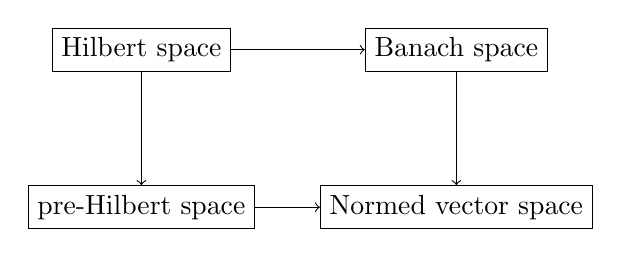
\begin{tikzpicture}[scale=2]
\node[rectangle, draw, fill=white] (N) at (2,0) {Normed vector space};
\node[rectangle, draw, fill=white] (P) at (0,0) {pre-Hilbert space};
\node[rectangle, draw, fill=white] (B) at (2,1) {Banach space};
\node[rectangle, draw, fill=white] (H) at (0,1) {Hilbert space};
\draw[->] (H) -- (B);
\draw[->] (H) -- (P);
\draw[->] (B) -- (N);
\draw[->] (P) -- (N);
\end{tikzpicture}
\end{center}
\end{figure}
\end{remark}

\begin{example}
  For any positive integer, the space $\R^n$ equipped with the
  Euclidean inner product
  \begin{gather*}
    \scal(x,y) = \sum_{i=1}^n x_i y_i
  \end{gather*}
  is a Hilbert space. The same holds for $\mathbb C^n$ and
  \begin{gather*}
    \scal(x,y) = \sum_{i=1}^n x_i \overline{y_i}.
  \end{gather*}
\end{example}

\begin{example}
  The spaces $\ell^2(\R)$ and $\ell^2(\mathbb C)$ of sequences
  $\{x_k\}_{k=1,\dots}$ of real and complex numbers, respectively, are
  Hilbert spaces, if equipped with the inner product
  \begin{gather*}
    \scal(x,y) = \sum_{i=k}^\infty x_k \overline{y_k}
    = \lim_{n\to\infty}\sum_{k=1}^n x_k \overline{y_k}.
  \end{gather*}
  An example for a sequence in $\ell^2(\R)$ is for instance the
  sequence $v = \{1/k\}_{k=1,\dots}$, since
  \begin{gather*}
    \norm{v}^2 = \sum_{k=1}^\infty \frac1{k^2} < \infty.
  \end{gather*}
  The sequence $w = \{1\}_{k=1,\dots}$ is not, since it does not converge
  quadratically.
\end{example}

\begin{Problem}{l2-Cauchy}
  Show that the sequence of sequences defined by
  \begin{gather*}
    v_n = \left\{1,\tfrac12,\dots,\tfrac1n,0,\dots,0\right\},
  \end{gather*}
  is a Cauchy sequence in $\ell^2$.
\end{Problem}

\begin{example}
  On the space of continuous functions on the interval
  $[-\pi/2,\pi/2]$ define the inner product
  \begin{gather*}
    \scal(f,g) = \int_{-\pi/2}^{\pi/2} f(x)g(x)\,dx.
  \end{gather*}
  Let
  \begin{gather*}
    V = \bigl\{f\in C[-\pi/2,\pi/2] \big| \scal(f,f) < \infty \bigr\}.
  \end{gather*}
  Then $V$ is a vector space with an inner product and thus a
  pre-Hilbert space, but it is not a Hilbert space, since for any $n$
  the sum
  \begin{gather*}
    f_n(x) = \frac4\pi \sum_{k=1}^n \frac{\sin\bigl((2k-1) x\bigr)}{2k-1}
  \end{gather*}
  is continuous, but
  \begin{gather*}
    \lim_{n\to\infty} f_n =
    \begin{cases}
      -1 & x<0 \\
      0 & x=0 \\
      1 & x>0
    \end{cases}
  \end{gather*}
  is not.
\end{example}

\begin{Definition}{separable}
  A subset $M$ of a Hilbert space $V$ is called \define{dense}, if
  every vector in $V$ is an accumulation point of $M$, that is, $V$ is
  the closure of $M$.  A Hilbert space is called \define{separable},
  if it has a countable dense subset.
\end{Definition}

\begin{todo}
\begin{remark}
  From the point of view of numerical analysis and computation, spaces
  which are not separable are of limited interest. In fact, every
  result of a numerical calculation is in a finite set. When we look
  at convergence for $n\to\infty$ or $h\to 0$, we are usually studying
  sequences with countable index sets. Therefore, vectors in
  nonseparable spaces cannot be approximated reliably.

  Apart from this remark, it is a goal of these notes to develop a
  framework for applied mathematics without recourse to the axiom of
  choice. Separable spaces allow us for instance to construct bases
  instead of deducing their existence indirectly.
\end{remark}
  I think this remark should be at the beginning of this chapter since
  here the idea behind these notes becomes clearer (to me). Also here,
  it some kind of disturbs the flow of the notes. Perhaps, if it is
  \emph{very} important to you, you could write a review at the end of
  the chapter stating the results and how your goals have been
  accomplished -- and maybe also \emph{why} this goal is so important.
\end{todo}

\begin{Definition}{schauder-basis}
  Let $V$ be a Hilbert space over a field $\mathbb K$. A
  \define{Schauder basis} or short \define{basis} of $V$ is a set
  $\{x_i\}$ of linearly independent vectors with coefficients $i$
  from an index set $I$, such that each $v\in V$ has a representation
  of the form
  \begin{gather*}
    v = \sum_{i\in I} \alpha_i x_i,
  \end{gather*}
  with coefficients $\alpha_i \in \mathbb K$. The index set $I$ may be
  finite in the case of a finite dimensional vector space, or
  countable if $V$ is infinite dimensional and separable. In the
  latter case it is required that the sum in the linear combination
  exists as the limit of a series. In particular, the sum must be a
  Cauchy-sequence with respect to the norm of $V$.
\end{Definition}

\begin{remark}
  In the infinite dimensional case, the norm of the vector space is
  part of the definition of the basis. This is the usual view in
  functional analysis, but it fails if no norm is defined on a general
  vector space $V$. In that case, only finite sums can be admitted,
  leading to a \define{Hamel basis}. While these seem to be more
  immediate extensions of bases on finite dimensional spaces, we will
  not have good use for them here.

  We will use the concept of orthogonality below to establish a
  general existence result for Schauder bases in Hilbert spaces.
\end{remark}

\begin{notation}
  We will use the term \putindex{sequence} to denote an at most
  countable set. The elements of a sequence are numbered by indices
  and the index set is $\mathbb N$ or a subset thereof.
\end{notation}

%%%%%%%%%%%%%%%%%%%%%%%%%%%%%%%%%%%%%%%%%%%%%%%%%%%%%%%%%%%%%%%%%%%%%%
%%%%%%%%%%%%%%%%%%%%%%%%%%%%%%%%%%%%%%%%%%%%%%%%%%%%%%%%%%%%%%%%%%%%%%
\section{Orthogonality}
%%%%%%%%%%%%%%%%%%%%%%%%%%%%%%%%%%%%%%%%%%%%%%%%%%%%%%%%%%%%%%%%%%%%%%
%%%%%%%%%%%%%%%%%%%%%%%%%%%%%%%%%%%%%%%%%%%%%%%%%%%%%%%%%%%%%%%%%%%%%%

\begin{Definition}{orthogonal}
  Let $V$ be an inner product space over a field $\mathbb K$. Two
  vectors $x,y\in V$ are called \define{orthogonal} if $\scal(x,y) = 0$. We
  write $x\perp y$. Let $W$ be a subspace of $V$. We say that a vector $v$
  is orthogonal to the subspace $W$, if it is orthogonal to every vector in
  $W$.

  A set of nonzero mutually orthogonal vectors
  $\{x_i\} \subset V$ is called \define{orthogonal set}. If
  additionally $\norm{x_i} = 1$ for all vectors, it is called an
  \define{orthonormal set}. These notions transfer directly from
  finite to countable sets.
\end{Definition}

\begin{Definition}{orthogonal-complement}
  Let $W\subset V$ be a subspace of a Hilbert space $V$. We define its
  \define{orthogonal complement} $\ortho W\subset V$ by
  \begin{gather}
    \label{eq:infsup:7}
    \ortho W = \bigl\{v\in V \big| \scal(v,w)_{V} = 0
    \;\forall\,w\in W\bigr\}.
  \end{gather}
\end{Definition}

\begin{Lemma}{orthogonal-closed}
  The orthogonal complement $\ortho W$ of a subspace $W\subset V$
  is closed in the sense of ~\slideref{Definition}{complete}.
\end{Lemma}

\begin{proof}
  By the \putindex{Bunyakovsky-Cauchy-Schwarz inequality}, the inner
  product is continuous on $V\times V$. Therefore, the mapping
  \begin{align*}
    \phi_w\colon V &\to \R,\\
    v&\mapsto \scal(v,w),
  \end{align*}
  is continuous. For any $w\in W$, the kernel of $\phi_w$ is closed as
  the pre-image of the closed set $\{0\}$. Since
  \begin{gather*}
    \ortho W = \bigcap_{w\in W} \ker{\phi_w},
  \end{gather*}
  it is closed as the intersection of closed sets.
\end{proof}

\begin{Theorem}{orthogonal-complement}
  Let $W$ be a subspace of a Hilbert space $V$ and $W^\perp$ its
  orthogonal complement. Then, $W^\perp = \overline{W}^\perp$. Further,
  $V = W \oplus W^\perp$ if and only if $W$ is closed.
\end{Theorem}

\begin{proof}
  Clearly, $\overline{W}^\perp \subset W^\perp$ since
  $W\subset\overline{W}$. Let now $u\in W^\perp$. Then, $\phi =
  \scal(u,\cdot)$ is a continuous linear functional on $V$. Therefore,
  if a sequence $w_n \subset W$ converges to $w\in \overline{W}$, we
  have
  \begin{gather*}
    \scal(u,w) = \lim_{n\to\infty} \scal(u,w_n) = 0,
  \end{gather*}
  since $u \in W^\perp$. Hence, $u\in \overline{W}^\perp$ and
  $W^\perp = \overline{W}^\perp$.

  Now, the ``only if'' follows by the fact, that if $W$ is not
  closed, there is an element $w\in \overline{W}$ but not in $W$ such that
  $\scal(w,u)=0$ for all $u\in W^\perp$. Thus, $w\not\in W^\perp$ and
  consequently $w\not\in W^\perp \oplus W$.

  Let now $W$ be closed. We show that for all $v \in V$ there is a unique
  decomposition
  \begin{gather}
    \label{eq:infsup:8}
    v = w + u,\qquad \text{with} \qquad w\in W, \;u\in W^\perp.
  \end{gather}
  This is equivalent to $V = W \oplus W^\perp$. Uniqueness follows,
  since
  \begin{gather*}
    v = w_1+u_1 = w_2+u_2
  \end{gather*}
  implies that for any $y\in V$
  \begin{gather*}
    0 = \scal(w_1-w_2+u_1-u_2,y) = \scal(w_1-w_2,y) + \scal(u_1-u_2,y).
  \end{gather*}
  Choosing $y=u_1-u_2$ and $w_1-w_2$ in turns, we see that one of the
  inner products vanishes for orthogonality and the other implies that
  the difference is zero.

  If $v\in W$, we choose $w=v$ and $u=0$. For $v\not\in W$, we prove
  existence by considering that due to the closedness of $W$ there holds
  \begin{gather*}
    d=\inf_{w' \in W} \norm{v-w'} >0.
  \end{gather*}
  Let $w_n$ be a minimizing sequence. Using the parallelogram identity
  \begin{gather*}
    \norm{a+b}^2+\norm{a-b}^2 = 2\norm{a}^2+2\norm{b}^2,
  \end{gather*}
  we prove that $\{w_n\}$ is a Cauchy sequence by
  \begin{align*}
    \norm{w_m-w_n}^2 &= \norm{(v-w_n)-(v-w_m)}^2\\
    &= 2\norm{v-w_n}^2+2\norm{v-w_m}^2-\norm{2v-w_m-w_n}^2\\
    &= 2\norm{v-w_n}^2+2\norm{v-w_m}^2-4\norm*{v-\frac{w_m+w_n}2}^2\\
    &\le 2\norm{v-w_n}^2+2\norm{v-w_m}^2-4d^2,
  \end{align*}
  since $(w_m+w_n)/2\in W$ and $d$ is the infimum. Now we use the
  minimizing property to obtain
  \begin{gather*}
    \lim_{m,n\to\infty}\norm{w_m-w_n}^2 = 2d^2+2d^2 -4d^2=0.
  \end{gather*}
  Since $V$ is given as a Hilbert space and as such complete, $w=\lim w_n$
  exists and by the closedness of $W$, we have $w\in W$. Let $u=v-w$.
  By continuity of the norm, we have $\norm{u}=d$. It remains to show
  that $u\in W^\perp$. To this end, we introduce the variation
  $w+\epsilon \tilde w$ with $\tilde w \in W$ to obtain
  \begin{align*}
    d^2 &\le \norm{v-w-\epsilon \tilde w}^2\\
    &= \norm{u}^2-2\epsilon\scal(u,\tilde w)+\epsilon^2 \norm{\tilde w},
  \end{align*}
  implying for any $\epsilon>0$
  \begin{gather*}
    0\le-2\epsilon\scal(u,\tilde w)+\epsilon^2 \norm{\tilde w},
  \end{gather*}
  which requires $\scal(u,\tilde w) = 0$. Since $\tilde w \in W$ was chosen
  arbitrarily, we have $u \in W^\perp$.
\end{proof}

\begin{Corollary}{ortho-density}
  A subspace $W$ of a Hilbert space $V$ is dense in $V$ if and only if
  $\ortho W = \{0\}$.
\end{Corollary}

\begin{proof}
  The ``only if'' is an immediate application of
  \slideref{Theorem}{orthogonal-complement}. For the opposite
  direction, assume $\overline W \neq V$. Choose $v\in V$ such that
  $v\not\in \overline W$. By
  \slideref{Theorem}{orthogonal-complement}, there are unique elements
  $w\in W$ and $u\in \ortho W$, such that $v=w+u$. In particular,
  $u\neq 0$.
  \begin{todo}
    Make this a lemma about  the fact that on the polar space!!
    Now, let $\phi = \scal(u,.) \in V^*$. Then, there holds
    \begin{align*}
      \phi(u) &= \norm{u}_V^2 \neq 0 \\
      \phi(w) &= 0 \quad\forall w\in W.
    \end{align*}
    Thus, from the fact that $W$ is not dense follows the existence of a
    linear functional which vanishes on $W$, but not on $V$.
  \end{todo}
\end{proof}

\begin{Definition}{ortho-projection}
  Let $W$ be a closed subspace of the Hilbert space $V$ and $\ortho W$
  be its orthogonal complement. Then, the
  \define{orthogonal projection} operators
  \begin{gather}
    \label{eq:lafa:9}
    \begin{split}
      \Pi_W &\colon V\to W\\
      \Pi_{\ortho W} &\colon V\to \ortho W\\
    \end{split}
  \end{gather}
  are defined by the unique decomposition
  \begin{gather}
    \label{eq:lafa:10}
    v = \Pi_W v + \Pi_{\ortho W} v.
  \end{gather}
\end{Definition}

\begin{Lemma*}{gram-schmidt}{Gram--Schmidt}
  For every linearly independent sequence of
  vectors $\{v_i\}$ there is an up to scaling unique orthonormal set
  $\{x_i\}$ with the property that
  \begin{gather*}
    \forall n\in \mathbb N:\quad
    \operatorname*{span}_{i=1,\dots,n} \{x_i\}
    =
    \operatorname*{span}_{i=1,\dots,n} \{v_i\}.
  \end{gather*}
\end{Lemma*}

\begin{proof}
  The proof uses induction over the length of the sequence.  Beginning
  with $v_1$, choose $x_1 = v_1$, which is nonzero by the assumption
  of linear independence.

  Assume now that the lemma holds for the elements $v_1,\dots,v_k$, such that
  \begin{gather*}
    V_k = \spann{v_1,\dots,v_k} = \spann{x_1,\dots,x_k}.
  \end{gather*}
  Again, by linear independence, $v_{k+1}$ is not in $V_k$ and $V_k$
  is closed since it is finite dimensional. Hence, we can choose
  \begin{gather*}
    \tilde x_{k+1} = \Pi_{\ortho V_k} v_{k+1},
    \qquad \frac{\tilde x_k}{\norm{\tilde x_k}}.
  \end{gather*}
\end{proof}

  
\begin{Theorem}{Hilbert-basis}
  Every separable Hilbert space has an at most countable, orthonormal
  Schauder basis.
\end{Theorem}

% See e.g.~\cite{Yosida80}.
\begin{proof}
  First, let $M$ be a countable dense subset
  of $V$, which exists due to the separability assumption. Now choose
  any numbering of $M$ and $v_1$ the first nonzero element in
  $M$. For $i=2,\dots,\infty$ choose with $v_1,\dots,v_{i-1}$ given
  $v_i$ as the next vector in $M$ which is not in the subspace spanned
  by $v_1,\dots,v_{i-1}$. This procedure generates an at most
  countable sequence $\{v_1, \dots, v_i\}_{i=1, \dots}$ of linearly
  independent vectors. It will only stop, if $V$ is finite dimensional.
  Furthermore, we have that every element in $M$ can be written as a finite
  linear combination of these vectors: Assume $w \in M$ as $w \not \in
  \spann{v_1,\dots,v_k}$ for any natural number $k$. Since $M$ is countable,
  we will eventually get to $w$ which then --- by definition of the sequence
  --- will be added to it as $v_{k+1} = w$.
  
  The sequence $\{v_i\}_{i=1,\dots}$ is a Schauder basis for $V$. In fact, given a
  vector $v\in V$ we have to show that for every $\epsilon$, there is
  a finite linear combination $s_n = \sum_{i=1}^n \alpha_i v_i$ such
  that $\norm{v-s_n} < \epsilon$. Let by separability $w_\epsilon$ be in
  $M$ such that $\norm{v-w_\epsilon} < \epsilon$. Since
  $w_\epsilon in M$, there is $n$ such that $s_n = w_\epsilon$.

  Finally, we use the Gram--Schmidt procedure to orthogonalize the
  sequence.
\end{proof}

\begin{Theorem}{Hilbert-basis-completion}
  Let $W$ be a closed subspace of a separable Hilbert space $V$ and
  $\{x_k\}$ be an orthonormal basis for $W$. Then, this basis can be
completed to be a basis of $V$.
\end{Theorem}

\begin{Problem}{Schauder-basis-completion}
  Prove \slideref{Theorem}{Hilbert-basis-completion}. Take into account
  that $W$ is not assumed finite dimensional.
\end{Problem}

\begin{example}
  In the Hilbert spaces $\R^n$, $\mathbb C^n$, $\ell^2(\R)$, and
  $\ell^2(\mathbb C)$, an orthonormal basis is obtained by choosing
  basis vectors $x_i$ with entries $x_{i,j} = \delta_{ij}$.
\end{example}

\begin{Lemma*}{Bessel-inequality}{Bessel inequality}
  Let $\{x_i\}$ be an orthonormal basis of the Hilbert space $V$. For
  $v\in V$, define %the \define{Fourier coefficient}s
  \begin{gather}
    \label{eq:lafa:18}
    \alpha_i = \scal(v,x_i), \qquad i=1,\dots
  \end{gather}
  Then,
  \begin{gather}
    \label{eq:lafa:18a}
    \sum_{i=1}^\infty \abs{\alpha_i}^2 \le \norm{v}_V^2.
  \end{gather}
\end{Lemma*}

\begin{proof}
  For $n\in \mathbb N$, we have
  \begin{align*}
    \norm*{v-\sum_{i=1}^n \alpha_i x_i}^2
    &= \scal(v-\sum \alpha_i x_i,v-\sum \alpha_i x_i) \\
    &= \norm{v}^2 -\scal(v,\sum \alpha_i x_i)
      -\scal(\sum \alpha_i x_i, v) + \sum \abs{\alpha_i}^2\\
    &= \norm{v}^2 - \sum \abs{\alpha_i}^2.
  \end{align*}
  Since the left hand side is nonnegative, the Bessel inequality holds.
\end{proof}

\begin{Lemma*}{Parseval-identity}{Parseval identity}
  Under the same assumptions as in \slideref{Lemma}{Bessel-inequality}
  the sequence
  \begin{gather*}
    f_n = \sum_{i=1}^n \alpha_i x_i = \sum_{i=1}^n \scal(f, x_i) x_i
  \end{gather*}
  converges to $f$ in $V$ and there holds
  \begin{gather}
    \label{eq:lafa:19}
    \norm{f}^2 = \sum_{i=1}^\infty \abs{\alpha_i}^2.
  \end{gather}
\end{Lemma*}

\begin{proof}   
  First, we will show that the series $\{f_n\}_{n=1,\dots}$ is a
  Cauchy sequence and, using the completeness of $V$, deduce that
  $\{f_n\}_{n=1,\dots}$ does indeed converge in $V$. Second, we will
  prove that indeed there holds $f_n \to f$ as $n \to \infty$.
  Finally, it is easy to show that $\norm{f}^2$ does indeed equal to
  $\sum_{i=1}^\infty \abs{\scal(f, x_i)}^2$.
  
  Take $m,\, n \in \mathbb{N}$ with $n>m$ and consider
  \begin{gather*}
    \norm{f_n - f_m}^2 = \norm{\sum_{i=m+1}^n \scal(f, x_i) x_i}^2.
  \end{gather*}
  Since $\{x_i\}_{i=1,\dots}$ are indeed pairwise orthogonal, we can
  use the Pythagorean Theorem to obtain that the above equation becomes
  \begin{gather*}
    \sum_{i=m+1}^n \norm{\scal(f, x_i) x_i}^2
      = \sum_{i=m+1}^n \abs{\scal(f, x_i)}^2  \norm{x_i}^2.
  \end{gather*}
  Furthermore, the $\{x_i\}_{i=1,\dots}$ are orthonormal. Hence,
  $\norm{x_i} = 1$ for all $i=1, \dots$. The above equation simplifies to
  \begin{gather*}
    \sum_{i=m+1}^n \abs{\scal(f, x_i)}^2.
  \end{gather*}
  By Bessel's inequality we know that
  \begin{gather*}
    \sum_{i=1}^\infty \abs{\scal(f, x_i)}^2 \le \norm{f}_V^2
  \end{gather*}
  and hence $\{f_n\}_{n=1,\dots}$ converges. Therefore, the difference
  $\norm{f_n - f_m}^2$ can be arbitrarily small and hence the sequence
  $\{f_n\}_{n=1,\dots}$ is Cauchy. Since $V$ is given as a Hilbert space,
  $V$ is also complete. By that, the sequence $\{f_n\}_{n=1,\dots}$
  converges to some $\bar{f} \in V$.
  
  To prove that $f = \bar{f}$, consider $\scal(f-\bar{f}, x_k)$ for some
  $k \in \mathbb{N}$. If we show that this equals zero, we know that
  $(f-\bar{f}) \perp x_k$ for any $k \in \mathbb{N}$. 
  By linearity of the inner product, we have that
  \begin{align*}
  \scal(f-\bar{f}, x_k) &= \scal(f, x_k)
    -\sum_{i=1}^\infty \scal(f, x_i)\scal(x_i, x_k) \\
    &= \scal(f, x_k) - \scal(f, x_k) = 0.
  \end{align*}
  Here we used that $\scal(x_i, x_k) = \delta_{i,k}$. Hence $(f-\bar{f})
  \perp x_k$. Since $\{x_k\}_{k=1,\dots}$ form a basis, there holds
  \begin{gather}
  \label{eq:lafa:18b}
  f = \bar{f} = \lim_{n\to \infty} \sum_{i=1}^n \scal(f, x_i) x_i.
  \end{gather}
  
  Finally, we have that
  \begin{gather*}
    \norm{f} = \norm{\lim_{n\to \infty} \sum_{i=1}^n \scal(f, x_i) x_i}.
  \end{gather*}
  By continuity of the norm and equation ~(\ref{eq:lafa:18b}) the above
  equation becomes
  \begin{gather*}
    \lim_{n\to \infty} \norm{\sum_{i=1}^n \scal(f, x_i) x_i}.
  \end{gather*}
  Using the Pythagorean theorem and the orthogornality we obtain
  \begin{gather*}
  \lim_{n\to \infty} \sum_{i=1}^n \abs{\scal(f, x_i)} \cdot 1
    = \sum_{i=1}^\infty \abs{\scal(f, x_i)}.
  \end{gather*}
  Thus, Parseval's identity has been established as desired.
\end{proof}

\begin{remark}
  In his monograph ``Mémoire sur les séries et sur l'intégration complète
  d'une équation aux différences partielles linéaires du second ordre,
  à coefficients constants'' from April 5, 1799, Marc-Antoine Parseval
  published his ``original'' identity for Fourier coefficients. The other
  ingredients for more more generalized formulation took some more time:
  In 1898, Guiseppe Peano came up with the theory of pre-Hilbert spaces,
  or, at that time, inner product spaces. In 1907, Riesz and Fischer
  (independently) came up with their famous theorem, the completeness of
  $L^p$ for $0<p \le \infty$ which has been used for $p=2$. The more
  general version of his theorem was published in Titchmarchs book in
  1939. In the meantime, someone must have connected the dots and found
  this more general formulation. Unfortunately, his/her name has apparently
  been forgotten.
\end{remark}

%%%%%%%%%%%%%%%%%%%%%%%%%%%%%%%%%%%%%%%%%%%%%%%%%%%%%%%%%%%%%%%%%%%%%%
%%%%%%%%%%%%%%%%%%%%%%%%%%%%%%%%%%%%%%%%%%%%%%%%%%%%%%%%%%%%%%%%%%%%%%
\section{Linear operators}
%%%%%%%%%%%%%%%%%%%%%%%%%%%%%%%%%%%%%%%%%%%%%%%%%%%%%%%%%%%%%%%%%%%%%%
%%%%%%%%%%%%%%%%%%%%%%%%%%%%%%%%%%%%%%%%%%%%%%%%%%%%%%%%%%%%%%%%%%%%%%

\begin{intro}
  Linear mappings are the next central topic of linear algebra, which
  we want to extend to infinite dimensional spaces. Here, the basic
  definition remains the same, that is, a \define{linear operator} is
  a mapping of a Hilbert space $V$ to a Hilbert space $W$ which is
  compatible with vector operations. But Hilbert spaces have
  additional structure by their norms and their completeness.
\end{intro}

\begin{Definition}{linear-operator}
  Let $V,W$ be two vector spaces. A \define{linear mapping} or
  \define{linear operator} $L\colon V\to W$ is a mapping such that
  \begin{gather*}
    L(\alpha u+\beta v) = \alpha L(u) + \beta L(v),
  \end{gather*}
  for all $\alpha,\beta\in\mathbb K$ and for all $u,v\in V$.
%  such that  $L(u)$ and $L(v)$ are defined.
\end{Definition}

\begin{Definition}{bounded-operator}
  A linear operator $L\colon V\to W$ is called \define{bounded} on $V$
  if there exists a constant $c$ such that
  \begin{gather}
    \label{eq:lafa:11}
    \norm{L v}_W \le c \norm{v}_V
    \quad\forall v\in V.
  \end{gather}
  We define the operator norm $\norm{L}$ as
  \begin{gather}
    \label{eq:lafa:12}
    \norm L = \sup_{v\in V} \frac{\norm{L v}_W}{\norm{v}_V}.
  \end{gather}
\end{Definition}

\begin{remark}
  Every linear mapping of a finite dimensional space is continuous,
  even \putindex{Lipschitz continuous}. This follows easily from the
  matrix representation. The fact that a linear mapping can be
  unbounded is a new property of infinite dimensional spaces, which
  will be discussed in §\ref{???}.
\end{remark}

\begin{Theorem}{continuous-operator}
  A linear operator $L\colon V\to W$ is continuous on $V$ if and only
  if it is bounded. It is continuous everywhere if it is continuous in
  a single point.
\end{Theorem}

\begin{todo}
\begin{proof}
  Let $L\colon V\to W$ be bounded with boundary constant $c$ and let
  the sequence $\{v_n\}_{n=1,\dots} \subset V$ converge to some 
  $v \in V$ as $n \to \infty$. Using the boundedness of $L$, we obtain
  \begin{gather*}
    \norm{Lv_n - Lv} = \norm{L(v_n - v)} \le c\norm{v_n - v}.
  \end{gather*}
  By the convergence of $\{v_n\}_{n=1,\dots}$ we get that $Lv_n \to Lv$
  as $n \to \infty$. Hence, $L$ is continous.
  
  Now assume $L$ as unbounded. Then, there exists a sequence
  $\{v_n\}_{n=1,\dots}$ such that $\norm{Lv_n}$ diverges as $n \to \infty$.
  Define the sequence $\{\tilde{v}_n\}_{n=1,\dots}$ as
  \begin{gather*}
    \tilde{v}_n = \frac{v_n}{\norm{Lv_n}}.
  \end{gather*}
  We immediately get that $\norm{L\tilde{v}_n} = 1$ for all $n$, but
  $\norm{\lim_{n\to\infty}L\tilde{v}_n} = 0$. Thus, $L$ is not continous.
  
  For the second equivalence note that continuity trvially implies
  continuity in a single point, e.g. $x \in V$. Now let $L$ be continous 
  n $x$ and take the sequence $\{v_n\}_{n=1,\dots} \subset V$ converging
  to $v \in V$ Then, $\{v_n-(v-x)\}_{n=1,\dots}$ converges to $x$ and by
  continuity we have $L(v_n-(v-x)) = Lv_n - Lv + Lx \to Lx$ as $n \to \infty$.
  This yields $Lv_n \to Lv$ and thus, $L$ is continous.
\end{proof}
\end{todo}

%%%%%%%%%%%%%%%%%%%%%%%%%%%%%%%%%%%%%%%%%%%%%%%%%%%%%%%%%%%%%%%%%%%%%%
%%%%%%%%%%%%%%%%%%%%%%%%%%%%%%%%%%%%%%%%%%%%%%%%%%%%%%%%%%%%%%%%%%%%%%
\section{The dual space}
%%%%%%%%%%%%%%%%%%%%%%%%%%%%%%%%%%%%%%%%%%%%%%%%%%%%%%%%%%%%%%%%%%%%%%
%%%%%%%%%%%%%%%%%%%%%%%%%%%%%%%%%%%%%%%%%%%%%%%%%%%%%%%%%%%%%%%%%%%%%%

\begin{Definition}{dual-space}
  A \define{linear functional} on a vector space $V$ is a
  \putindex{linear mapping} from $V$ to $\mathbb K$.

  The \define{dual space} $V^*$ of a vector space $V$, also called the
  \define{normed dual}, is the space of all bounded linear functionals
  on $V$ equipped with the norm
  \begin{gather}
    \norm{\phi}_{V^*} = \sup_{v\in V} \frac{\phi(v)}{\norm{v}_V}.
  \end{gather}
\end{Definition}

\begin{intro}
  From linear algebra, we know that the dual of $\R^n$ is $\R^n$
  itself, and for every basis $\{e_1,\dots,e_n\}$ we can define a dual
  basis $\{d_1,\dots,d_n\}$ by the conditions
  \begin{gather*}
    d_i(e_j) = \delta_{ij}.
  \end{gather*}
  The following results establish similar results for general Hilbert
  spaces.
\end{intro}

\begin{Theorem*}{Riesz-representation}{Riesz representation theorem}
  Let $V$ be a Hilbert space. Then, $V$ is isometrically isomorphic to
  $V^*$. In particular, there is an isomorphism
  \begin{gather}
    \label{eq:lafa:1}
    \begin{split}
      \varrho\colon V & \to V^*, \\
      y & \mapsto f,
    \end{split}
  \end{gather}
  such that
  \begin{gather}
    \label{eq:lafa:2}
    \begin{split}
    \scal(x,y) &= f(x) \qquad \forall x\in V,\\
    \norm{y}_V &= \norm{f}_{V^*}.
    \end{split}
  \end{gather}
  We refer to $\varrho$ as \define{Riesz isomorphism}.
\end{Theorem*}

% from Yosida III.6
\begin{proof}
  The proof is constructive and makes use of the orthogonal
  complement.

  First, it is clear that for any $y\in V$ a linear functional
  $f\in V^*$ is defined by $f(\cdot) = \scal(y,\cdot)$. Furthermore,
  $\varrho$ is injective, since
  \begin{gather*}
    \scal(x,y) = 0 \qquad\forall x\in V
  \end{gather*}
  implies $y\in \ortho V = \{0\}$. By the
  \putindex{Bunyakovsky-Cauchy-Schwarz inequality}, we have
  \begin{gather*}
    \norm{f}_{V^*} = \sup_{x\in V}\frac{\abs{f(x)}}{\norm{x}_V}
    = \sup_{x\in V}\frac{\abs{\scal(x,y)}}{\norm{x}_V}
      \le \norm{y}_V,
  \end{gather*}
  with equality for $x=y$.  It remains to show that $\varrho$ is
  surjective. To this end, let $f\in V^*$ be arbitrary and let
  $N = \ker f$. If $N=V$, we choose $y=0$. If not, choose
  $\ortho y \in \ortho N$ and let
  \begin{gather}
    \label{eq:lafa:13}
    y = \frac{\overline{f(\ortho y)}}{\norm*{\ortho y}^2} \ortho y \in
    \ortho N,
  \end{gather}
  such that $f(y) = \abs*{f(\ortho y)}^2/\norm*{\ortho y}^2 \neq 0$.
  Let now $x\in V$ be chosen arbitrarily. Then, there holds
  \begin{gather*}
    x = \left(x-\frac{f(x)}{f(y)} y\right)
    + \frac{f(x)}{f(y)} y.
    \\
  \end{gather*}
  Since
  \begin{gather*}
      f = \left(x-\frac{f(x)}{f(y)} y\right) 
      = \left(f(x)-f(x) \frac{f(y)}{f(y)}\right)
      = 0,
  \end{gather*}
  this decomposition amounts to $x = x^0+\ortho x$ with $x^0\in N$ and
  $\ortho x \in \ortho N$. It is unique according to
  \slideref{Definition}{ortho-projection}. Thus, we have that $\ortho x$ is a
  multiple of $y$, say $\ortho x=\alpha y$ and thus
  \begin{gather*}
    \begin{aligned}
    f(x) &= f(x^0) + f(\ortho x)
    &=& \alpha f(y)
    &=& \alpha \frac{\abs*{f(\ortho y)}^2}{\norm*{\ortho y}^2}
    \\
    \scal(x,y) &= \scal(x^0,y)  + \scal(\ortho x,y)
    &=& \alpha \norm{y}_V^2
    &=& \alpha \frac{\abs*{f(\ortho y)}^2}{\norm*{\ortho y}^4}
    \norm*{\ortho y}^2
    \end{aligned}
  \end{gather*}
  Hence, the two terms are equal and $\varrho$ is surjective.
\end{proof}

%%%%%%%%%%%%%%%%%%%%%%%%%%%%%%%%%%%%%%%%%%%%%%%%%%%%%%%%%%%%%%%%%%%%%%
%%%%%%%%%%%%%%%%%%%%%%%%%%%%%%%%%%%%%%%%%%%%%%%%%%%%%%%%%%%%%%%%%%%%%%
\section{Weak convergence and compact operators}

\begin{example}
  Let $\phi:\ell^2(\R)\to\ell^2(\R)$ be such that
  \begin{gather*}
    v =
    \begin{pmatrix}
      x_1 \\ x_2 \\ \vdots \\ x_k \\ \vdots
    \end{pmatrix}
    \mapsto \phi(v) =
    \begin{pmatrix}
      x_1 \\ 4x_2 \\ \vdots \\ k^2x_k \\ \vdots
    \end{pmatrix}.
  \end{gather*}
  Clearly, $\phi$ is linear. But if we consider the sequence of
  vectors $v_n = \{\delta_{nk}\}$, we see that $v_n \mapsto n^2 v_n$ and
  thus, while the sequence is bounded in $\ell^2(\R)$, its image is
  not.
  
  Moreover, take now the sequence of sequences
  \begin{gather*}
    v_n = \left\{1,\tfrac12,\dots,\tfrac1n,0,\dots,0\right\}
    \quad \mapsto \quad \phi(v_n) = \{1,2,\dots,n,0,\dots,0\}.
  \end{gather*}
  The sequence $v_n$ converges to a limit $v \in \ell^2(\R)$, while
  the sequence $\phi(v_n)$ diverges. While $\phi(v_n)$ is defined for
  all $v_n$, it is not bounded for the limit $v$.
\end{example}

\begin{remark}
  By virtue of completeness of the space, whenever a linear operator
  is not bounded, it must be undefined for some vectors. We could
  exclude such operators from our considerations, but we would
  severely limit the theory we want to develop. Instead, we will
  accept the fact, that we have to extend the notion of a linear
  mapping $\phi: V\to W$ to a linear operator $\phi: V\to W$, which
  may not be defined on all of $V$. The following definition fixes
  this problem somewhat.
\end{remark}

\begin{Definition}{operator-domain}
  Let $\phi: V\to W$ be a linear operator. Then, the \define{domain}
  of $\phi$ is
  \begin{gather*}
    \mathcal D(\phi) = \bigl\{ v\in V \big|
    \phi(v) \in W \bigr\}.
  \end{gather*}
  Here, $\phi(v) \in W$ implies that $\phi(v)$ is also well defined.
\end{Definition}

%%%%%%%%%%%%%%%%%%%%%%%%%%%%%%%%%%%%%%%%%%%%%%%%%%%%%%%%%%%%%%%%%%%%%%
%%%%%%%%%%%%%%%%%%%%%%%%%%%%%%%%%%%%%%%%%%%%%%%%%%%%%%%%%%%%%%%%%%%%%%
\section{Unbounded linear operators}


%%% Local Variables: 
%%% mode: latex
%%% TeX-master: "main"
%%% End: 


\chapter{Iterative methods in finite and infinite dimensional spaces}

\svnid{$Id$}

\begin{remark}
  This part of the notes deals with preconditioning of symmetric
  operators, or those, which have a dominating symmetric part. The
  theory of preconditioning methods for nonsymmetric and in particular
  non-normal operators is currently barely developed and thus cannot
  be covered by these notes. 
\end{remark}

\begin{example}
  While the methods developed in this chapter are fairly general, we
  introduce a specific model problem as a simple benchmark case. To
  this end, we consider the Dirichlet problem: find $u\in V =
  H^1_0(\Omega)$ such that
  \begin{gather}
    \label{eq:itintro:1}
    a(u,v) \equiv \int_\Omega \nabla u\cdot \nabla v \dx
    = \int_\Omega f v \dx \equiv f(v),
    \qquad \forall v\in V.
  \end{gather}
  The finite dimensional linear systems of equations are derived from
  finite element discretizations on quasi-uniform meshes of cells with
  maximal diameter $h$, yielding a sequence of spaces $V_h$, on which
  linear systems are introduced by the same weak
  form~\eqref{eq:itintro:1}.
\end{example}

\begin{notation}
  With a bilinear form $a(.,.)$ on $V\times V$ we associate the
  operator $A: V\to V^*$ by
  \begin{gather}
    \label{eq:itintro:2}
    \scal(Au,v) = a(u,v), \quad \forall v\in V,
  \end{gather}
  where $\scal(.,.):V^*\times V \to \R$ is the canonical bilinear form of an
  element of $V^*$ and an element of $V$, namely
  \begin{gather}
    \label{eq:richardson:9}
    \scal(f,v) = f(v), \quad \forall f\in V^*, v\in V.
  \end{gather}
  
  We will tacitly assume that operators $A$, $B$, etc.\ are defined by
  equation~\eqref{eq:itintro:2} and the bilinear forms $a(.,.)$,
  $b(.,.)$, etc., respectively, if they are not defined otherwise.
  
  After choosing a basis for a finite dimensional space $V_n$ or a
  Schauder basis for the space $V$ (assuming $V$ separable), say
  $\{\phi_i\}$, we can define a (possibly infinite-dimensional) matrix
  $\mat A$ associated with the bilinear form $a(.,.)$ with the entries
  \begin{gather*}
    a_{ij} = a(\phi_j, \phi_i).
  \end{gather*}
  
  If we restrict the bilinear forms to a finite dimensional subspace
  $V_n$, we denote the matrices $\mat A$ restricted to this subspace
  by $\mat A_n$. Accordingly, we define the bounds
  \begin{gather}
    \label{eq:richardson:8}
    \Lambda_n = \max_{u\in V_n}\frac{a(u,u)}{\norm{u}_V^2},
    \qquad
    \lambda_n = \min_{u\in V_n}\frac{a(u,u)}{\norm{u}_V^2}.
  \end{gather}
\end{notation}

%%% Local Variables: 
%%% mode: latex
%%% TeX-master: "main"
%%% End: 

\svnid{$Id$}

\section{The Richardson iteration}

\begin{intro}
  As a first example and prototype for all other iterative methods we
  consider Richardson's method, which for matrices and vectors in
  $\R^n$ reads
  \begin{gather}
    \label{eq:richardson:1}
    \vec x^{(k+1)}
    = \vec x^{(k)}
    - \omega_k \bigl(\mat A \vec x^{(k)} - \vec b \bigr).
  \end{gather}
  $\omega_k$ is a relaxation parameter, which can be chosen a priori
  or can be changed in every step. We will for simplicity assume
  $\omega_k = \omega$.
\end{intro}  

\begin{theorem}
  \label{theorem:richardson:1}
  If $\mat A$ is symmetric, positive definite, with extremal
  eigenvalues $\lambda>0$ and $\Lambda>0$, then Richardson's method
  converges if and only if $0 < \omega < 2/\Lambda$. The optimal
  relaxation parameter is 
  \begin{gather}
    \label{eq:richardson:2}
    \omega_{\text{opt}} = \frac{2}{\lambda+\Lambda},
  \end{gather}
  which yields an optimal contraction rate of
  \begin{gather}
    \label{eq:richardson:4}
    \rho_{\text{opt}}
    = 1-\frac{2\lambda}{\lambda+\Lambda}
    = \frac{\Lambda-\lambda}{\Lambda+\lambda}
    = \frac{\kappa-1}{\kappa+1}
    = 1 -\frac2\kappa + \mathcal
    O\left(\kappa^{-2}\right),
  \end{gather}
  where $\kappa = \Lambda/\lambda$ is the so called \define{spectral
    condition number}.
\end{theorem}

\begin{proof}
  Convergence of this method is analyzed through the \putindex{Banach
    fixed-point theorem}, which requires contraction
  property of the matrix $\mat M = \mat I - \omega \mat A$.
  Alternatively, we studied a theorem that
  states, that a matrix iteration converges if and only if the
  spectral radius
  \begin{gather*}
    \rho(\mat M) = \max \left|\lambda(\mat M)\right| < 1,
  \end{gather*}
  the maximum absolute value of the eigenvalues of $\mat M$ is
  strictly less than one.
  
  If $\mat A$ is symmetric, positive definite, with eigenvalues
  $\lambda_i > 0$, we have that
  \begin{gather}
    \label{eq:richardson:13}
    \rho(\mat M) = \max_i \left|1-\omega \lambda_i\right|.
  \end{gather}
  Let the extremal eigenvalues be determined by the minimum and
  maximum of the Rayleigh quotient,
  \begin{gather}
    \label{eq:richardson:3}
    \lambda
    = \min_{x\in \R^n} \frac{\vec x^T\mat A\vec x}{\vec x^T\vec x},
    \qquad\text{and}\qquad
    \Lambda = \max_{x\in \R^n} \frac{\vec x^T\mat A\vec x}{\vec x^T\vec x}.
  \end{gather}
  Then, equation~\eqref{eq:richardson:13} yields that the method
  converges for $0 < \omega < 2/\Lambda$. Furthermore, for 
  $1/\Lambda \le \omega \le 2/\Lambda$ we have
  \begin{gather*}
    \rho(\mat M) = \max \bigl\{ -1+\omega \Lambda,  1-\omega \lambda \bigr\}.
  \end{gather*}
  The optimal parameter $\omega$ is the one where both values are
  equal and thus~\eqref{eq:richardson:2} and~\eqref{eq:richardson:4} hold.
\end{proof}

\begin{intro}
  The analysis of finite element methods shows that it is beneficial
  to give up the focus on finite dimensional spaces and rather use
  theory that applies to separable Hilbert spaces. If results can
  obtained in this context, they can easily be restricted to finite
  dimensional subspaces and thus become uniform with respect to the
  mesh parameter. Thus, we will first reformulate Richardson's method
  for this case and then derive convergence estimates.
\end{intro}

\begin{intro}
  Elements of an abstract Hilbert space $V$ will be denoted by
  $u,v,w$, etc. On the other hand, coefficient vectors in $\R^n$ are
  denoted by letters $\vec x,\vec y,\vec z$, etc.
\end{intro}

\begin{definition}
  Let $V$ be a Hilbert space with inner product $\scal(.,.)_V$. Let
  $a(.,.)$ be a second bilinear form on $V$. Then, for any right hand
  side $f\in V^*$ and any start vector $u^{(0)}\in V$,
  \define{Richardson's method} is defined by the iteration
  \begin{gather}
    \label{eq:richardson:5}
    \scal(u^{(k+1)},v)_V = \scal(u^{(k)},v)_V
    - \omega_k \bigl(a(u^{(k)},v) - f(v)\bigr), \qquad \forall v\in V.
  \end{gather}
  $\omega_k$ is a suitable \putindex{relaxation parameter}, chosen
  such that the method converges.
\end{definition}

\begin{note}
  The scalar products in~\eqref{eq:richardson:5} become necessary,
  since different from the case in $\R^n$, the result of applying the
  bilinear form $a(.,.)$ to $u^{(k)}$ in the first argument yields a
  linear form on $V$. In order to convert this to a vector in $V$, we
  have to apply the isomorphism induced by the \putindex{Riesz
    representation theorem}.
\end{note}

\begin{theorem}
  \label{theorem:richardson:2}
  Let the bilinear form $a(.,.)$ be bounded and elliptic on $V\times
  V$, namely, let there exist positive constants $\Lambda$ and $\lambda$ such
  that for all $u,v\in V$ there holds
  \begin{gather}
    \label{eq:richardson:6}
    a(u,v) \le \Lambda \norm{u}_V \norm{v}_V,
    \qquad
    a(u,u) \ge \lambda \norm{u}_V^2.
  \end{gather}
  Then, Richardson's iteration converges for
  $\omega_k = \omega$ for any $\omega \in (0, 2\lambda/\Lambda^2)$.
\end{theorem}

\begin{proof}
  We define the iteration operator $T$ as the solution operator of
  equation~\eqref{eq:richardson:5}, namely $T u^{(k)} := u^{(k+1)}$. We
  have to prove that $T$ is a contraction on $V$ under the assumptions
  of the theorem.

  For two arbitrary vectors $u^1, u^2 \in V$, let $w = u^1-u^2$ be
  their difference. Due to linearity, we have $T w = T u^1-T u^2$ and
  \begin{gather*}
    \scal(T w,v)_V = \scal(w,v)_V - \omega a(w,v) = \scal(w-\omega A w,v)_V.
  \end{gather*}
  Using $v=Tw$ as a test function, we obtain
  \begin{align*}
    \norm{Tw}_V^2
    & = \scal(w-\omega A w,w-\omega A w)_V \\
    &= \norm{w}_V^2 - 2\omega a(w,w) + \omega^2 \norm{Aw}_V^2\\
    & \le \norm{w}_V^2 - 2\lambda\omega \norm{w}_V^2
    +  \Lambda^2 \omega^2\norm{w}_V^2\\
    & = \underbrace{\bigl(1-2\lambda\omega
      + \Lambda^2\omega^2\bigr)}_{=:\rho(\omega)} \norm{w}_V^2.
  \end{align*}
  The function $\rho(\omega)$ is a parabola open to the top, which
  at zero equals one and has a negative derivative. Thus, it is less
  than one for small positive valuers of $\omega$. The other
  point where $\rho(\omega) = 1$ is $\omega = 2\lambda/\Lambda^2$.
\end{proof}

\begin{note}
  The condition on $\omega$ in Theorem~\ref{theorem:richardson:2} is
  more restrictive than in Theorem~\ref{theorem:richardson:1}, since
  $\lambda/\Lambda \le 1$. This is
  due to the fact, that in Theorem~\ref{theorem:richardson:1} we
  assume symmetry, and thus orthogonal diagonalizability of the matrix
  $\mat A$. With similar assumptions,
  Theorem~\ref{theorem:richardson:2} could be made sharper.
\end{note}

\begin{note}
  It is clear that the boundedness and ellipticity
  estimates~\eqref{eq:richardson:6} hold for any finite dimensional
  subspace $V_n\subset V$, and thus the convergence
  estimate~\eqref{eq:richardson:4} becomes independent of $n$.
  
  More interesting and also more common is the case where the bilinear form
  $a(.,.)$ is unbounded on $V$. While it is still bounded on each
  finite subspace $V_n$, this bound cannot be independent of $n$ if
  the sequence $\{V_n\}$ approximates $V$.
\end{note}  

\begin{note}
  We define an operator $B:V\to V^*$ such that $Bu = b(u,.) :=
  \scal(u,.)_V$. By the Riesz representation theorem, there is a
  continuous inverse operator $B^{-1}: V^*\to V$, which is often
  called \define{Riesz isomorphism}.
\end{note}

\begin{definition}
  When we apply Richardson's method as in~\eqref{eq:richardson:5} on a
  computer, each step involves a multiplication with the matrix $\mat A$,
  but an inversion of the matrix $\mat B$, corresponding to the iteration
  \begin{gather*}
    \mat B \vec x^{(k+1)}
    = \mat B \vec x^{(k)}
    - \omega_k \bigl(\mat A \vec x^{(k)} - \vec b \bigr),
  \end{gather*}
  or equivalently,
  \begin{gather}
    \label{eq:richardson:7}
    \vec x^{(k+1)}
    = \vec x^{(k)}
    - \omega_k \mat B^{-1}\bigl(\mat A \vec x^{(k)} - \vec b \bigr).
  \end{gather}
  The iteration in~\eqref{eq:richardson:7} is commonly referred to as
  \define{preconditioned Richardson iteration} and $\mat B^{-1}$ as the
  \define{preconditioner}. Note that by introducing the iteration in
  its weak form~\eqref{eq:richardson:5}, the preconditioner arrives
  naturally and with necessity.
  
  The goal of this chapter is finding preconditioners $\mat B^{-1}$, or
  equivalently inner products $\scal(.,.)_V$, such that the bilinear
  form $a(.,.)$ is bounded and the condition number
  $\kappa = \Lambda/\lambda$ is small.
  
  In order to reduce (or increase) confusion, we will refer to the
  inner product that we search in order to bund the condition number
  as $b(.,.)$ instead of $\scal(.,.)_V$, this way separating the
  Hilbert space $V$ more clearly from the task of
  preconditioning. Thus, the operator $B$ and the matrix $\mat B$ will
  be associated with a bilinear form $b(.,.)$ and the final version of
  the preconditioned Richardson iteration in the space $V$ is
  \begin{gather}
    \label{eq:richardson:10}
    b(u^{(k+1)},v)_V = b(u^{(k)},v)_V
    - \omega_k \bigl(a(u^{(k)},v) - f(v)\bigr), \qquad \forall v\in V,
  \end{gather}
  or in operator form
  \begin{gather}
    \label{eq:richardson:11}
    u^{(k+1)} = u^{(k)} - \omega_k B^{-1} (A u^{(k)} - f).
  \end{gather}
\end{definition}

\begin{corollary}
  Let the symmetric bilinear forms $a(.,.)$ and $b(.,.)$ in the
  Richardson iteration~\eqref{eq:richardson:10} fulfill the
  \define{spectral equivalence} relation
  \begin{gather}
    \label{eq:richardson:12}
    \lambda b(u,u) \le a(u,u) \le \Lambda b(u,u), \quad \forall u\in V.
  \end{gather}
  Then, if $\omega_k \equiv \omega \in (0,2\Lambda)$, the iteration is
  a contraction on $V$. The optimal contraction number is $\rho$
  according to equation~\eqref{eq:richardson:4} for $\omega$ chosen as
  in~\eqref{eq:richardson:2}.
\end{corollary}

\begin{proof}
  This corollary is equivalent to Theorem~\ref{theorem:richardson:2}
  if the inner product $\scal(.,.)_V$ is replaced by the bilinear form
  $b(.,.)$.
\end{proof}

\begin{notation}
  \index{lambdaBA@$\lambda(B,A)$}
  \index{Lambdaba@$\Lambda(B,A)$}
  In order to distinguish different preconditioners, we will also us
  the notation $\lambda(B, A)$ and $\Lambda(B,A)$ to refer to the
  constants in the norm equivalence~\eqref{eq:richardson:12}.
\end{notation}


\begin{example}
  Let us take the example~\eqref{eq:itintro:1}.
  By the Poincaré-Friedrichs inequality, $a(.,.)$ is an inner product
  on $V$ and thus we can choose $\scal(.,.)_V = a(.,.)$. In
  particular, $\lambda = \Lambda = 1$ and the optimal choice is
  $\omega = 1$. Then, Richardson's iteration becomes
  \begin{gather*}
    a(u^{(k+1)},v) = a(u^{(k)},v)
    - \bigl(a(u^{(k)},v) - f(v)\bigr) =  f(v), \qquad \forall v\in V,
  \end{gather*}
  which converges in a single step, but we have to solve the original
  equation for $u$. Thus, either the inversion of the matrix $A_n$ is
  trivial on each finite dimensional subspace $V_n$, or the method is
  useless. With usual finite element bases, the latter is true.
\end{example}

\begin{example}
  In the other extreme, we would like to use the $\R^n$ or $L^2$
  inner product on $V_n$ or $V$, such that the Riesz isomorphism is
  easily computable. But then, the bilinear form $a(.,.)$ is unbounded
  on $V$. Thus, while for each finite $n$, the condition number
  $\kappa_n = \Lambda_n/\lambda_n$ exists, it converges to infinity if
  $n\to\infty$.
\end{example}

\begin{todo}
  Show that the condition number grows like $1/h^2$ for finite element
  methods.
\end{todo}

%%% Local Variables: 
%%% mode: latex
%%% TeX-master: "main"
%%% End: 

\svnid{$Id$}

\section{The conjugate gradient method}

\begin{intro}
  Relying on Hilbert space structure more than Richardson's iteration
  is the \putindex{conjugate gradient method} (cg), since it uses
  orthogonal search directions. Nevertheless, it also relies on
  constructing search directions from residuals, such that a
  \putindex{Riesz isomorphism} enters the same way as before and can
  then be used for preconditioning.
  
  The beauty of the conjugate gradient method is, that it is parameter
  and tuning free, and it converges considerably faster than a linear
  iteration method.
\end{intro}

\begin{definition}[Conjugate gradient method]
  Let $V$ be a Hilbert space and $V^*$ its dual. The \define{conjugate
  gradient method} for an iteration vector $u^{(k)} \in V$ involves the
  residuals $r^{(k)} \in V^*$ as well as the update direction $p^{(k)}
  \in V$ and the auxiliary vector $w^{(k)} \in V$. It consists of the
  steps
  \begin{enumerate}
  \item Initialization: for $f$ and $u^{(0)}$ given, compute
    \begin{xalignat*}{2}
      r^{(0)} &= f- a(u^{(0)},.) \\
      \scal(w^{(0)}, v) &= r^{(0)}(v) & \forall v &\in V \\
      p^{(0)} &= w^{(0)}.
    \end{xalignat*}
    \item Iteration step: for $u^{(k)}$, $r^{(k)}$, $w^{(k)}$, and
      $p^{(k)}$ given, compute
      \begin{xalignat*}2
        \alpha_k &= \frac{r^{(k)}(w^{(k)})}{a(p^{(k)},p^{(k)})} \\
        u^{(k+1)} &= u^{(k)} + \alpha_k p^{(k)} \\
        r^{(k+1)} &= r^{(k)} - \alpha_k a(p^{(k)},.) \\
      \scal(w^{(k+1)}, v) &= r^{(k+1)}(v) & \forall v &\in V \\
      \beta_k &= \frac{r^{(k+1)}(w^{(k+1)})}{r^{(k)}(w^{(k)})}\\
      p^{(k+1)} &= w^{(k+1)} + \beta_k p^{(k)}
      \end{xalignat*}
  \end{enumerate}
\end{definition}

\begin{remark}
  The results on orthogonality and minimization properties of the cg
  method in~\cite{GrossmannRoosStynes07} or~\cite{Saad00} remain valid in this
  context. Differences occur in the interpretation of these
  properties. The conjugate gradient method does not necessarily
  converge in a finite number of steps, and if the bilinear form is
  unbounded, no convergence rate is guaranteed.
\end{remark}



% \begin{lemma}
%   Let $a(.,.)$ be symmetric and elliptic. Then, either $u^{(k)}$ is a
%   solution, or $u^{(k+1)}$ can be computed by a step of the conjugate
%   gradient method. Furthermore, there are the 
% \end{lemma}

\begin{definition}
  The \define{preconditioned cg method} is obtained from
  above algorithm by reinterpreting the \putindex{Riesz isomorphism}
  in the computation of $w^{(k+1)}$ as a preconditioning operation,
  much alike Definition~\ref{definition:richardson:2} of the
  preconditioned Richardson iteration. Thus, the line defining
  $w^{(k+1)}$ is replaced by
  \begin{xalignat*}2
    b(w^{(k+1)}, v) &= r^{(k+1)}(v) & \forall v &\in V .
  \end{xalignat*}
  Here, like there, the preconditioner enters naturally from the weak
  form of the algorithm.
\end{definition}

\begin{definition}
  The $n$th \define{Krylov space} as subspace of the Hilbert space $V$
  with inner product $b(.,.)$ of the operator $A$ and seed vector
  $w \in V$ is
  \begin{gather}
    \label{eq:cg:2}
    \mathcal K_n = \mathcal K_n(B^{-1}A, w)
    = \operatorname{span}\left\{w, B^{-1}A w, (B^{-1}A)^2 w, \dots, (B^{-1}A w)^{n-1}\right\}.
  \end{gather}
\end{definition}

\begin{lemma}
  The iterates of the cg method have the following minimization
  properties:
  \begin{gather}
    \label{eq:cg:3}
    \begin{split}
      \norm{u^{(k)}-u}_A &= \min_{v\in \mathcal K_k} \norm{u^{(0)} + v -u}_A \\
      &= \min_{\substack{p\in P_{n-1}\\ p(0) = 1}}
      \norm{u^{(0)} + p(B^{-1}A) w -u}_A.
    \end{split}
  \end{gather}
\end{lemma}

\begin{theorem}
  Let the bilinear form $a(.,.)$ be symmetric, and let the
  \putindex{spectral equivalence}~\eqref{eq:richardson:12} hold. Then,
  the preconditioned cg method converges and we have the estimate
  \begin{gather}
    \label{eq:cg:1}
    \|u^{(k)} - u\|_A \le 2
    \left(\frac{\sqrt\kappa-1}{\sqrt\kappa+1}\right)^k \|u^{(0)} - u\|_A.
  \end{gather}
  Here, $\kappa = \Lambda/\lambda$ is the \putindex{spectral condition
    number} of the preconditioned problem.
\end{theorem}

%%% Local Variables: 
%%% mode: latex
%%% TeX-master: "main"
%%% End: 


\chapter{Schwarz methods}
\label{cha:iteration:schwarz-methods}

\section{Additive Schwarz methods}

\begin{intro}
  In this section, we study preconditioners, which are related to
  subspace decompositions of the space $V$ or its finite dimensional
  subspaces. We will develop the theory in an abstract way, but always
  keep the model problem~\eqref{eq:itintro:1} in mind when we do so. In
  particular, the subspaces chosen will be associated with either
  coarser mesh levels or with meshes on subdomains of $\Omega$.
  
  This section follows in part~\cite[Chapter 7]{BrennerScott02}. A
  more detailed discussion with extension of the methods developed
  here can be found in~\cite{ToselliWidlund05}
\end{intro}

\subsection{The abstract framework}

\begin{intro}
  Let $V$ be a Hilbert space with inner product $\scal(.,.)$ and let
  $a(.,.): V\times V$ be a symmetric and $V$-elliptic not necessarily
  bounded bilinear form. Let a set of subspaces
  $\{V_j\}_{j=1,\dots,J}$ of $V$ be chosen such that
  \begin{gather*}
    V = \sum_{j=1}^J V_j.
  \end{gather*}
  The sum is not required to be direct, that is, a vector $v\in V$ may
  have several decompositions $v = \sum \alpha_j v_j$ with
  $v_j\in V_j$. Methods below based on the subspaces $V_j$ are called
  \define{subspace correction} methods.

  Alternatively, we consider methods based on abstract auxiliary
  spaces $\hat V_j$, such that
  \begin{gather*}
    V = \sum_{j=1}^J R_j^T \hat V_j,
  \end{gather*}
  where $R_j^T$ is an operator embedding the auxiliary space
  $\hat V_j$ into $V$.  Such methods are called \define{auxiliary
    space methods}. Subspace correction and auxiliary space methods
  are equivalent by considering $V_j = R_j^T \hat V_j$.
\end{intro}

\begin{assumption}
  \label{lemma:schwarz:1}
  There are bilinear forms $a_j(.,.)$ defined on $V_j$ such that the weak formulation
  \begin{gather}
    \label{eq:schwarz:1}
    a_j(u_j,v_j) = f(v_j),
    \quad\forall v_j\in V_j,
  \end{gather}
  has a unique solution $u_j\in V_j$ for all $f\in V_j^*$. In the
  context of auxiliary space methods, we assume that there are
  bilinear forms $\hat a_j(.,.)$ defined on $\hat V_j$ such
  that the weak formulation
  \begin{gather}
    \label{eq:schwarz:1a}
    \hat a_j(u_j,v_j) = f(v_j),
    \quad\forall v_j\in \hat V_j,
  \end{gather}
  has a unique solution $u_j\in \hat V_j$ for all $f\in \hat V_j^*$.
\end{assumption}

\begin{Definition}{subspace-projection}
  \label{definition:schwarz:1}
  \index{Pj@$P_j$|see {Ritz projection}} Let the \define{subspace
    projection} operator $P_j: V \to V_j$ be defined such that
  $P_j u \in V_j$ is the unique (Assumption~\ref{lemma:schwarz:1})
  solution to the problem
  \begin{gather}
    \label{eq:schwarz:2}
    a_j(P_j u,v_j) = a(u,v_j),\quad\forall v_j\in V_j.
  \end{gather}
  Note that this is a projection only if $a_j(.,.)$ is the restriction
  of the bilinear form $a(.,.)$ to the subspace $V_j$. In this
  case,\index{A-orthogonal projection@$A$-orthogonal projection|see
    {Ritz projection}} we call $P_j$ the $A$-orthogonal projection or
  \define{Ritz projection} to $V_j$. If $a_j(.,.)$ is not the
  restriction of $a(.,.)$, the operator $P_j$ still maps into $V_j$,
  but it is not idempotent.

  Since $V_j$ is a subspace of $V$, we will also understand $P_j$ as
  an endomorphism of $V$ iteself. The left hand side of this equation
  induces an operator $A_j: V_j \to V_j^*$ by $A_j u_j = a_j(u_j,.)$.
\end{Definition}

\begin{Definition}{auxiliary-space-projection}
  \label{definition:schwarz:1a}
  Let the operator $\hat P_j: V \to \hat V_j$ be defined such that $\hat P_j u \in \hat V_j$ is
  the unique (Assumption~\ref{lemma:schwarz:1}) solution to the problem
  \begin{gather}
    \label{eq:schwarz:2a}
    \hat a_j(\hat P_j u,v_j) = a(u,R_j^T v_j),\quad\forall v_j\in \hat V_j.
  \end{gather}
  The left hand side of this equation induces an operator $\hat A_j:
  \hat V_j \to \hat V_j^*$ by $\hat A_j u_j = \hat a_j(u_j,.)$.
\end{Definition}

\begin{Lemma}{schwarz-ritz}
  \label{lemma:schwarz:ritz}
  If the local bilinear forms $a_j(.,.)$ are the restrictions of
  $a(.,.)$ to $V_j$, then the projections $P_j$ as mappings from $V$
  to itself are self-adjoint with respect to the $a(.,.)$-inner
  product and positive semi-definite. Furthermore, $P_j$ acts as
  identity on $P_j$ and there holds $P_j^2 = P_j$.
\end{Lemma}
\begin{proof}
  This is a well-known fact about orthogonal projections, which we
  will prove shortly.
  First, we note that by the uniqueness in
  Lemma~\ref{lemma:schwarz:1} $P_j u_j = u_j$
  for all $u_j\in V_j$. Thus, for all $u\in V$: $P_j P_j u = P_j u$.
  Let now $u,v\in V$ arbitrary. Then, there holds
  \begin{gather*}
    a(u, P_j v) = a(P_j u, P_j v) = a(P_j v, P_j u)
    = a(v, P_j u) = a(P_j u, v).
  \end{gather*}
  Furthermore,
  \begin{gather*}
    a(P_j u,u) = a(u, P_j u) = a(P_j u, P_j u)\ge 0,
  \end{gather*}
  since $a(.,.)$ is positive definite.
\end{proof}

\begin{Definition}{l2-projection}
  \label{definition:schwarz:1a}
  For subspace and auxiliary space methods, we define the operators
  \begin{gather}
    \begin{split}
      \Pi_j: V &\to V_j\\
      R_j: V &\to\hat V_j
    \end{split}
  \end{gather}
  \index{Pij@$\Pi_j$}
  such that $\Pi_j u\in V_j$ is the solution to the problem
  \begin{gather}
    \scal(\Pi_j u_j,v_j) = \scal(u,v_j),\quad\forall v_j\in V_j.
  \end{gather}

  For auxiliary spaces $\hat V_j$, we define the projection like
  operators  through
  \begin{gather}
    \scal(R_j u_j,v_j)_{\hat V_j} = \scal(u,R_j^T v_j),\quad\forall v_j\in \hat V_j.
  \end{gather}
  
  % \index{Pijt@$\Pi^T_j$}
  % We define its dual $\Pi_j^T: V_j^* \to V^*$ by
  % \begin{gather}
  %   \label{eq:schwarz:3}
  %   \scal(\Pi_j^T \phi_j,v)_{V^*\times V} =  \scal( \phi_j,\Pi_j
  %   v)_{V_j^*\times V_j}
  % \end{gather}
\end{Definition}

% \begin{todo}
%   Show that $\Pi^T$ is an orthogonal projection, and onto which space.
% \end{todo}

\begin{Lemma}{schwarz-ritz-representation}
  \label{lemma:schwarz:2}  
  There holds
  \begin{gather}
    \label{eq:schwarz:15}
    A_j P_j = \Pi^T_j A.
  \end{gather}
\end{Lemma}

\begin{proof}
  Let $u,v\in V$ arbitrary. Let $v_j=\Pi_j v$. We rewrite
  equation~\eqref{eq:schwarz:2} as
  \begin{gather*}
    \scal(A_j P_j u, v)_{V^*\times V}
    = \scal(A_j P_j u, v_j)_{V^*\times V}
    = \scal(A u, v_j)_{V^*\times V}
    = \scal(\Pi^T_j A u, v)_{V^*\times V}.
  \end{gather*}
\end{proof}

\begin{Definition}{additive-schwarz}
  The \define{additive Schwarz preconditioner} for the operator $A$ associated
  with the symmetric, and $V$-elliptic bilinear form $a(.,.)$ with
  respect to the subspace decomposition $V_j$ is the mapping $B:
  V \to V^*$ such that
  \begin{gather}
    \label{eq:schwarz:4}
    B^{-1} = \sum_{j=1}^J P_j A^{-1}.
  \end{gather}
\end{Definition}

\begin{example}
  \label{example:schwarz:Jacobi}
  The \putindex{Jacobi method} may serve as a guiding example for the
  definition of these methods. To this end, let $V = \R^n$ with its
  Euclidean inner product $\scal(.,.)$. let $V_j =
  \operatorname{span}\{e_j\}$ be the space spanned by the $j$th unit
  vector. Let $A$ be a symmetric, positive definite matrix and $a(u,v)
  = v^T A u$. Then, equation~\eqref{eq:schwarz:2} becomes
  \begin{gather}
    \label{eq:schwarz:27}
    e_j^T A u_j = e_j^T A u
    \quad \Leftrightarrow \quad
    P_j u = u_j = \frac1{a_{j j}}(A u)_j.
  \end{gather}
  Since for this decomposition, the sum $V=\bigoplus V_j$ is direct,
  we obtain with $D=\operatorname{diag}(a_{11},\dots,a_{n n})$ the
  matrix representation
  \begin{gather*}
    (B^{-1} v)_j = \frac1{a_{j j}}(A A^{-1} v)_j = \frac1{a_{j j}} v_j
    \quad \Leftrightarrow \quad
    B^{-1} = D^{-1}.
  \end{gather*}
  We enter this preconditioner into the Richardson method in operator
  form~\eqref{eq:richardson:11} to obtain the iteration
  \begin{gather}
    \label{eq:schwarz:28}
    \begin{split}
      u^{(k+1)} &= u^{(k)} - \omega_k \sum_{j=1}^J P_j \bigl(u^{(k)} -
      A^{-1}f\bigr)\\
      &= u^{(k)} - \omega_k D^{-1} \bigl(A u^{(k)} - f\bigr).
    \end{split}
  \end{gather}
\end{example}

\begin{Lemma}{additive-positive-definite}
  \label{lemma:schwarz:3}
  If $A$ is symmetric and positive definite, so is $B^{-1}$ as defined
  in~\eqref{eq:schwarz:4}.
\end{Lemma}

\begin{proof}
  By Lemma~\ref{lemma:schwarz:2} and the fact that $P_j$ maps into $V_j$, we have that
  \begin{gather}
    \label{eq:schwarz:16}
    B^{-1} = \sum_{j=1}^J A_j^{-1} \Pi^T_j.
  \end{gather}
  Due to equation~\eqref{eq:schwarz:1}, $A_j$ inherits its symmetry
  and positive definiteness from $A$, and thus $A_j^{-1}$ is s.p.d.
  Therefore, for each term in this sum and arbitrary elements
  $\phi,\psi\in V^*$, we have
  \begin{gather*}
    \scal(A_j^{-1} \Pi^T_j \phi, \psi)_{V\times V^*}
    = \scal(A_j^{-1} \Pi^T_j \phi, \Pi^T_j \psi)_{V\times V^*}
    = \scal(\Pi^T_j \phi, A_j^{-1}\Pi^T_j \psi)
    = \scal(\phi, A_j^{-1}\Pi^T_j \psi).
  \end{gather*}
  The result now follows by linearity.
\end{proof}

\begin{Lemma}{additive-minimum}
  \label{lemma:schwarz:5}
  For $v\in V$ holds
  \begin{gather}
    \label{eq:schwarz:5}
    b(v,v) \equiv \scal(B v,v) = \min_{v=\sum v_j} \sum_{j=1}^J a(v_j,v_j),
  \end{gather}
  where the minimum is taken over all possible decompositions of $v$
  into a sum of elements $v_j\in V_j$ with $j=1,\dots,J$.
\end{Lemma}

\begin{proof}
  Since $B^{-1}$ is s.p.d., so is $B$. Therefore, $\scal(.,A_j^{-1}.)$
  is an inner product on $V_j^*$, for which the \putindex{Bunyakovsky-Cauchy-Schwarz
  inequality} holds. Thus, for an arbitrary decomposition $v=\sum v_j$
  with $v_j\in V_j$, the computation
  \begin{align*}
    b(v,v)
    &= \sum_{j=1}^J b(v, A_j^{-1} A_j v_j)
    = \sum_{j=1}^J \scal(\Pi^T_j B v, A_j^{-1} A_j v_j) \\
    &\le \sum_{j=1}^J \sqrt{\scal(\Pi^T_j B v, A_j^{-1}\Pi^T_j B v)}
    \sqrt{\scal(A_j v_j, A_j^{-1}A_j v_j)} \\
    & \le \sqrt{\sum_{j=1}^J \scal(\Pi^T_j B v, A_j^{-1}\Pi^T_j
      B v) }
    \sqrt{\sum_{j=1}^J \scal(A_j v_j,A_j^{-1}A_j v_j)} \\
    &= \sqrt{\scal(B v, {\sum A_j^{-1}\Pi^T_j} B v)}
    \sqrt{\sum_{j=1}^J \scal(A_j v_j, v_j)} \\
    &= \sqrt{b(v,v)} \sqrt{\sum_{j=1}^J a(v_j, v_j)},
  \end{align*}
  yields for arbitrary decompositions
  \begin{gather}
    \label{eq:schwarz:17}
    b(v,v) \le \sum_{j=1}^J a(v_j, v_j),
  \end{gather}
  and thus in particular, that the left hand side is bounded by the
  minimum of the right. Now we choose a special decomposition, showing
  that it cannot be less than the minimum. To this end, let
  \begin{gather}
    \label{eq:schwarz:18}
    v_j = A_j^{-1} \Pi^T_j B v.
  \end{gather}
  By Lemma~\ref{lemma:schwarz:2}, we have
  \begin{gather*}
    \sum v_j = \sum A_j^{-1} \Pi^T_j B v = B^{-1} B v = v.
  \end{gather*}
  Furthermore,
  \begin{align*}
    \sum_{j=1}^J \scal(A_j v_j, v_j)
    &= \sum_{j=1}^J \scal(A_j A_j^{-1} \Pi^T_j B v, A_j^{-1} \Pi^T_j
    B v) \\
    &= \sum_{j=1}^J \scal(\Pi^T_j B v, A_j^{-1} \Pi^T_j v) \\
    &= \scal(B v, \sum A_j^{-1} \Pi^T_j B v) = b(v, v).
  \end{align*}
\end{proof}

\begin{Theorem}{schwarz-equivalence}
  \label{theorem:schwarz:1}
  Let $A$ be s.p.d. and $B$ defined by
  equation~\eqref{eq:schwarz:4}. Then, the \putindex{spectral
    equivalence}~\eqref{eq:richardson:12} holds with
  positive constants
  \begin{gather}
    \label{eq:schwarz:19}
%    \begin{split}
    \Lambda(B,A) = \max_{v\in V} \frac{a(v,v)}{\min\limits_{v=\sum v_j}
      \sum\limits_{j=1}^J a(v_j, v_j)}
    ,\qquad
    \lambda(B,A) = \min\limits_{v\in V} \frac{a(v,v)}{\min\limits_{v=\sum v_j}
      \sum\limits_{j=1}^J a(v_j, v_j)}.
%    \end{split}
  \end{gather}
\end{Theorem}

\begin{proof}
  Here we use the fact, that $b(.,.)$ is an inner product on
  $V$ and that by
  \begin{gather*}
    b(B^{-1}A v,v) = a(v,v) = b(v, B^{-1}A v),
  \end{gather*}
  the operator $B^{-1}A$ is symmetric with respect to this inner
  product. Thus, the \putindex{Rayleigh quotient} qualifies to
  estimate the extremal eigenvalues, for instance,
  \begin{gather*}
    \Lambda(B^{-1}A)
    = \max_{v\in V} \frac{b(B^{-1}A v,v)}{b(v,v)}
    = \max_{v\in V} \frac{a(v,v)}{\min\limits_{v=\sum v_j}
      \sum\limits_{j=1}^J a(v_j, v_j)},
  \end{gather*}
  and the same for the minimum.
\end{proof}

\begin{note}
  \label{note:schwarz:1}
  In order to estimate the condition number $\Lambda(B,A)/\lambda(B,A)$ of a Schwarz
  preconditioner, it is now sufficient to bound the two quotients
  in~\eqref{eq:schwarz:19} from above and below. In particular, in
  order to find a bound for $\Lambda(B,A)$, we have to find an estimate of
  the form
  \begin{gather}
    \label{eq:schwarz:23}
    a(v,v) \lesssim \min_{v=\sum v_j}\sum_{j=1}^J a(v_j, v_j),
  \end{gather}
  or in other words, $a(v,v)$ has to be bounded by the sum on the
  right for any decomposition $v=\sum v_j$. On the other hand, in
  order to bound $1/\lambda(B,A)$, we need an estimate in the opposite direction,
  where it is sufficient to find one decomposition $v=\sum v_j$ such
  that it holds. We reduce these
  conditions to the following two abstract assumptions, which guarantee that
  Theorem~\ref{theorem:schwarz:1} holds true.
\end{note}

\begin{assumption}[Stable decomposition]
  \label{assumption:schwarz:stable-decomposition}
  For each $v\in V$ there is a decomposition
  \begin{gather*}
    v = \sum_{j=1^J} v_j, \qquad v_j\in V_j,
  \end{gather*}
  such that there holds
  \begin{gather}
    \label{eq:schwarz:24}
     \min_{v=\sum v_j}\sum_{j=1}^J a(v_j, v_j) \lesssim a(v,v).
  \end{gather}  
\end{assumption}

\begin{assumption}[Strengthened Cauchy-Schwarz inequalities]
  \label{assumption:schwarz:1}
  \defindex{strengthened Cauchy-Schwarz inequalities}
  \index{E@$\mathcal E$} There is a symmetric $J\times J$-matrix
  $\mathcal E$ with entries $\epsilon_{ij} \in [0,1]$ and a constant
  $C$ independent of $J$, such that for the spectral radius
  $\rho(\mathcal E)$ there holds
  \begin{gather*}
    \rho(\mathcal E) \le C
  \end{gather*}
  and for all $1 \le i,j \le J$, $v_i \in V_i$ and $v_j \in V_j$ there
  holds
  \begin{gather}
    \label{eq:schwarz:25}
    \left| a(v_i, v_j)\right|
    \le \epsilon_{ij} \sqrt{a(v_i,v_{\phantom ji})} \sqrt{a(v_j,v_j)}.
  \end{gather}
\end{assumption}

\begin{note}
  Inequality~\eqref{eq:schwarz:25} with $\epsilon_{ij} \equiv 1$ holds by the
  regular \putindex{Bunyakovsky-Cauchy-Schwarz inequality}.
  But for such a matrix, the
  spectral radius is $J$. As the following lemma will reveal, it is
  necessary to obtain $\rho(\mathcal E)$ independent of $J$ to obtain
  estimate~\eqref{eq:schwarz:23}.
\end{note}

\begin{Lemma}{schwarz-maximum}
  \label{lemma:schwarz:7}
  Let the estimate~\eqref{eq:schwarz:25} hold. Then,
  estimate~\eqref{eq:schwarz:23} holds with the constant
  $\rho(\mathcal E)$.
\end{Lemma}

\begin{proof}
  Let $v\in V$ and its decomposition $v=\sum v_j$ with $v_j\in V_j$ be
  chosen arbitrarily. Then,
  \begin{multline*}
    a(v,v)
    = a\left(\sum_i v_i, \sum_j v_j\right)
    = \sum_{i,j=1}^J a(v_i, v_j)
    \le \sum_{i,j=1}^J \epsilon_{ij} \sqrt{a(v_{\vphantom{j}i},v_i)} \sqrt{a(v_j,v_j)}.
  \end{multline*}
  The latter sum corresponds to a matrix-vector product of the form
  $\vec x^T \mathcal E \vec x$, where the entries of $x$ are of the
  form $\sqrt{a(v_i,v_i)}$. Since $\mathcal E$ is symmetric positive
  definite, this product can be estimated by $\rho(\mathcal E) |\vec
  x|^2$, and thus
  \begin{gather}
    \label{eq:schwarz:38}
    a(v,v) \le \rho(\mathcal E) \sum_{j=1}^J a(v_j,v_j).
  \end{gather}
\end{proof}

%%%%%%%%%%%%%%%%%%%%%%%%%%%%%%%%%%%%%%%%%%%%%%%%%%%%%%%%%%%%%%%%%%%%%%
%%%%%%%%%%%%%%%%%%%%%%%%%%%%%%%%%%%%%%%%%%%%%%%%%%%%%%%%%%%%%%%%%%%%%%
\section{Two-level additive Schwarz preconditioner}
%%%%%%%%%%%%%%%%%%%%%%%%%%%%%%%%%%%%%%%%%%%%%%%%%%%%%%%%%%%%%%%%%%%%%%
%%%%%%%%%%%%%%%%%%%%%%%%%%%%%%%%%%%%%%%%%%%%%%%%%%%%%%%%%%%%%%%%%%%%%%

\begin{intro}
  This preconditioner is in the class of \putindex{domain
    decomposition} methods. The attribute \putindex{two-level} refers
  to the fact that we are considering finite element discretizations
  of~\eqref{eq:itintro:1} on two finite element meshes, the
  \putindex{fine mesh} $\T_h$ on which we desire to compute the
  solution, and the auxiliary \putindex{coarse mesh} $\T_H$. Both
  meshes cover the whole domain $\Omega$ (see
  Figure~\ref{fig:schwarz:ddmeshes}), and each cell of the coarse mesh
  is the union of cells of the fine mesh ($4\times 4$ fine cells in
  the figure).

  In addition to these two meshes, we introduce subdomains
  $\Omega_1,\Omega_2,\dots,\Omega_J$ of $\Omega$ such that each
  $\Omega_j$ is the union of cells in $\T_h$. We require that those
  subdomains overlap each other like the three examples in
  Figure~\ref{fig:schwarz:ddmeshes} on the right. A more precise
  definition of the required overlap follows.
\end{intro}

\begin{figure}[tp]
  \centering
  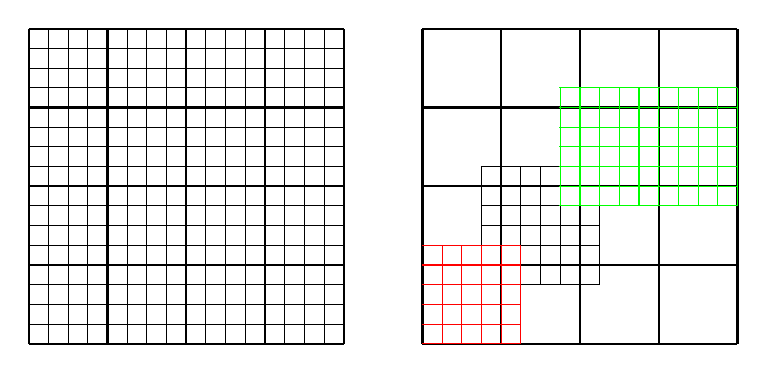
\begin{tikzpicture}
    \draw[step=.25cm] (-2,-2) grid (2,2);
    \draw[step=1cm,thick] (-2,-2) grid (2,2);
    \draw[step=1cm,thick] (3,-2) grid (7,2);
    \draw[step=.25cm] (3.74,-1.25) grid (5.25,0.25);
    \draw[step=.25cm,red] (3,-2) grid (4.25,-0.75);
    \draw[step=.25cm,green] (4.74,-0.25) grid (7,1.25);
  \end{tikzpicture}
  \caption{Fine mesh and coarse mesh (left) for overlapping domain
    decomposition. Examples for a subdomain decomposition on the
    right.}
  \label{fig:schwarz:ddmeshes}
\end{figure}

\begin{definition}{dd-overlap}
  \label{definition:schwarz:overlap}
  A covering of $\Omega$ with subdomains $\Omega_j$ is called
  \define{overlapping} with minimal \define{overlap} $\delta$, if for
  each $\Omega_j$ and all $x\in\Omega_j$ holds:
  \begin{gather*}
    \operatorname{dist}(x,\partial\Omega_J\setminus\partial\Omega) <
    \delta\;
    \Rightarrow\; \exists k\neq j: x\in \Omega_k.
  \end{gather*}
\end{definition}

\begin{Definition}{dd-finite-covering}
  \label{definition:schwarz:finite-covering}
\defindex{NO@$N_O$}
  \defindex{finite covering}
  We say that a family of coverings is finite, if
  there is a constant $N_O$ independent of $\T_h$ and the number of
  subdomains, such that for each $j$ the intersection
  $\Omega_j\cap\Omega_k$ is nonempty for at most $N_O$ subdomains
  $\Omega_k$.
\end{Definition}

\begin{Definition}{partition-of-unity}
  A smooth \define{partition of unity} with respect to the subdomains
  $\Omega_1,\Omega_2,\dots,\Omega_J$ of $\Omega$ is a set of
  nonnegative functions $\{\phi_1,\dots,\phi_J\}\subset
  C^\infty(\overline\Omega)$ such that
  \begin{xalignat}2
    \label{eq:schwarz:6}
    \phi_j(x) &  = 0
    & \forall x & \in \Omega\setminus\Omega_j, \quad j=1,\dots,J
    \\
    \label{eq:schwarz:7}
    \sum_{j=1}^J \phi_j(x) &= 1
    & \forall x&\in\overline\Omega.
  \end{xalignat}
  Similarly, we can define partitions of unity in $H^1(\Omega)$ or
  partitions of unity which are piecewise $C^1$.
  
  Furthermore, we assume that there is a positive constant $\delta$,
  called \define{overlap}, such that for all $j=1,\dots,J$ there holds
  \begin{gather}
    \label{eq:schwarz:8}
    \norm{\nabla\phi j}_{L^\infty(\Omega)} \lesssim \frac 1\delta,
  \end{gather}
  where the implicit constant is independent of $h$, $\delta$ and $J$.
\end{Definition}

\begin{note}
  The term overlap for $\delta$ is justified by the following
  consideration. Let $x \in \Omega_j$ be a point which is not in any
  other $\Omega_i$. Then, $\phi_j(x) = 1$. If~\eqref{eq:schwarz:8} is
  to hold, then it is necessary that
  $\operatorname{dist}(x,\partial\Omega_J) \ge \delta$ (up to a
  constant, but this constant is already
  in~\eqref{eq:schwarz:8}). Thus, the points of distance less than
  $\delta$ from $\partial\Omega_j$ must be elements of another
  subdomain as well, which is then said to overlap with $\Omega_j$.
\end{note}

\begin{example}
  \label{example:schwarz:2}
  On uniform meshes, overlapping subdomains with an overlap of
  $\delta = n h$ with $n=1,2,\ldots$ can be achieved easily by the
  following procedure:
  \begin{enumerate}
  \item Begin with a non overlapping subdivision $\{\Omega_j^0\}$,
    for instance aligned with the mesh cells of $\T_H$.
  \item Add all cells that share at least a vertex with a cell in
    $\Omega_j^0$ to obtain a domain $\Omega_j^1$. After this
    procedure, two neighboring domains will overlap by two cells,
    resulting in $\delta = 2h$.
  \item Repeat this procedure to obtain larger overlaps.
  \end{enumerate}
  
  On the resulting partitions, a partition of unity in $H^1$ can be
  constructed with piecewise linear (bilinear on quadrilaterals)
  functions. For instance for $\Omega_j^1$ this function is
  constructed as follows:
  \begin{enumerate}
  \item Choose $\phi_j(x) = 1/2$ in all vertices on $\partial \Omega_j^0$.
  \item Choose $\phi_j(x) = 0$ in all vertices on $\partial \Omega_j^1$ and outside
    $\Omega_j^1$.
  \item Choose $\phi_j(x) = 1$ in all remaining vertices inside
    $\Omega_j^0$.
    \item Connect these values by linear (on simplicial meshes), bilinear
      (quadrilateral meshes) of trilinear (hexahedral meshes)
      polynomials inside each mesh cell $T\in \T_h$.
  \end{enumerate}
  This partition of unity achieves the estimate~\eqref{eq:schwarz:8}
  with a constant of $1/2$.
\end{example}

\begin{notation}
  \label{par:schwarz:1}
  The solution space of our problem is the space $V=V_h$ given by the
  finite element space on the mesh $\T_h$. We define finite element
  spaces on $\Omega_j$ by
  \begin{gather}
    \label{eq:schwarz:9}
    V_j = \bigl\{ v\in V_h \big| \forall x\in\Omega\setminus\Omega_j :
    v(x) =0\bigr\}.
  \end{gather}
  Additionally, we define the space $V_0 \equiv V_H$ as the finite
  element space on the coarse mesh $\T_H$.  Since the meshes are
  nested, $V_H$ is indeed a subspace of $V_h$. Thus, we obtain a
  decomposition of $V_h$ into $J+1$ subspaces
  \begin{gather*}
    V_h = V_0 + \sum_{j=1}^J V_j,
  \end{gather*}
  where the last $J$ are associated with the subdomains. In fact,
  Lemma~\ref{lemma:schwarz:4} below states that already the spaces
  $V_1$ to $V_J$ are sufficient to span $V_h$. Nevertheless, the
  coarse grid space plays a crucial role in the efficiency of the
  method due to Lemma~\ref{lemma:schwarz:stable-decomposition}.
\end{notation}

\begin{Definition}{two-level-additive}
  Let the spaces $V_j$, $j=0,\dots,J$ be defined as above. Then, the
  \define{two-level additive Schwarz preconditioner} is defined as
  \begin{gather}
    \label{eq:schwarz:10}
    B^{-1}_{\text{TLS}} = \sum_{j=0}^J P_j A^{-1} = \sum_{j=0}^J A_j^{-1} \Pi^T_j,
  \end{gather}
  where $P_j$ is defined according to~\eqref{eq:schwarz:2} and $A_j:
  V_j\to V_j^*$ by
  \begin{gather}
    \scal(A_j u_j, v_j)_V = a(u_j, v_j),\quad\forall u_j, v_j \in V_j.
  \end{gather}
\end{Definition}

\begin{note}
  In order to simplify notation, we have assigned index zero to
  $V_H$. Thus, sums in future terms may either start at one, summing
  over subdomains, or at zero, summing over all subspaces.
\end{note}

\begin{Lemma}{schwarz4}
  \label{lemma:schwarz:4}
  There holds
  \begin{gather}
    \label{eq:schwarz:11}
    V_h = \sum_{j=1}^J V_j.
  \end{gather}
\end{Lemma}

\begin{proof}
  Let $I_h: C(\overline\Omega) \to V_h$ be the interpolation operator
  of the finite element space. Then, for any given $v\in V_h$ define
  $v_j = I_h(\phi_j v)$, where $\phi_j$ is the function associated to
  $\Omega_j$ of a partition of unity for $\Omega_1,\dots,\Omega_J$.
  
  By definition of $\phi_j$, there holds $\phi_j v = 0$ on
  $\Omega\setminus\Omega_j$. Furthermore, we assumed that a mesh cell
  of $\T_h$ is either completely in $\Omega_j$ or completely in its
  complement. Since nodal values of a cell are located in the cell
  itself, this implies that $I_h (\phi_j v) = 0$ on
  $\Omega\setminus\Omega_j$. Therefore, $I_h (\phi_j v) \in V_j$.
  
  On the other hand, we use the linearity of the interpolation
  operator to obtain
  \begin{gather*}
    \sum_{j=1}^J v_j = \sum_{j=1}^J I_h(\phi_j v)
    = I_h\left(v\sum_{j=1}^J \phi_h\right)
    = I_h v = v,
  \end{gather*}
  thus, the $v_j$ are indeed a decomposition of $v$. Since $v\in V_h$
  was chosen arbitrarily, the lemma is proven.
\end{proof}

\begin{Lemma}{finite-overlap-cauchy-schwarz}
  \label{lemma:schwarz:8}
  Let the covering $\{\Omega_j\}_{j=1,\dots,J}$ for $\Omega$ be finite
  according to
  Definition~\ref{definition:schwarz:finite-covering}. Then, the
  \putindex{strengthened Cauchy-Schwarz inequalities}~\eqref{eq:schwarz:25} hold
  with a spectral radius
  \begin{gather}
    \label{eq:schwarz:26}
    \rho(\mathcal E) \le N_O.
  \end{gather}
\end{Lemma}

\begin{proof}
  The term $a(v_i, v_j)$ is nonzero only if the supports of the two
  functions have a nonempty intersection. Accordingly, for each index
  $i$ only a maximum of $N_O$ of the coefficients $\epsilon_{ij}$ are
  nonzero. We set these equal to one and use Gershgorin's theorem to
  estimate the greatest eigenvalue.
\end{proof}

\begin{Lemma}{two-level-bound1}
  \label{lemma:schwarz:6}
  Let $v_j\in V_j$ for $j=0,\dots,J$ be a composition of $v\in V_h$
  such that
  \begin{gather*}
    v=\sum_{j=0}^J v_j.
  \end{gather*}
  Then,
  \begin{gather}
    \label{eq:schwarz:12}
    a(v,v) \lesssim \sum_{j=0}^J a(v_j, v_j),
  \end{gather}
  where the implicit constant does not depend on $h$, $H$, or $J$.
\end{Lemma}

\begin{proof}
  First a note: the inequality would be obvious, if $V_h$ was a direct
  sum of the spaces $V_j$, and it would hold with a constant of one if
  they were mutually orthogonal. Thus, we have to show some kind of
  orthogonality between the spaces.

  We start out by stating that
  \begin{align*}
    a(v,v) &= a\left(v_0+\sum_{j=1}^J v_j, v_0+\sum_{j=1}^J v_j\right)
    \\
    &\le 2 \left(a(v_0, v_0) + a\!\left(\sum_{j=1}^J v_j,\sum_{j=1}^J
        v_j\right)\right)
    \\
    &= 2 \left(a(v_0, v_0) + \sum_{j,k=1}^J a(v_j,v_k)\right) \\
    & \le 2 a(v_0, v_0) + 2 N_O \sum_{j=0}^J a(v_j, v_j),
  \end{align*}
  where the last inequality is due to Lemma~\ref{lemma:schwarz:7} and
  Lemma~\ref{lemma:schwarz:8}. Since $N_O$ is assumed independent of
  $h$, $H$, and $J$, the lemma is proven.
\end{proof}


\begin{Lemma}{stable-decomposition}
  \index{stable decomposition}
  \label{lemma:schwarz:stable-decomposition}
  For each $v\in V_h$ there exists a decomposition $v=\sum_{j=0}^J
  v_j$ with $v_j\in V_j$, such that
  \begin{gather}
    \label{eq:schwarz:13}
    \sum_{j=0}^J a(v_j, v_j)
    \lesssim \left(1+\frac H\delta\right)^2 a(v,v).
  \end{gather}
\end{Lemma}

\begin{proof}
  Let $\tilde I_H: H^1_0(\Omega) \to V_H$ be an interpolation operator
  continuous on $H^1(\Omega)$, for instance the interpolation operator
  by Clement or the one by Scott and Zhang. For a given function
  $v\in V_h$, let $v_H = \tilde I_H v$. Then
  \begin{gather}
    \label{eq:schwarz:20}
    \begin{split}
      |v_H|_1 &\lesssim |v|_1 \\
      \norm{v-v_H}_0 &\lesssim H |v|_1.
    \end{split}
  \end{gather}
  From~\eqref{eq:schwarz:20} there holds
  \begin{gather}
    \label{eq:schwarz:22}
    a(v_H,v_H) = |v_H|_1^2 \lesssim |v|_1^2 = a(v,v).
  \end{gather}
  Let $w=v-v_H$. Using a partition of unity $\{\phi_j\}$ for the
  subdomains $\{\Omega_j\}$ and the nodal interpolant $I_h$ as in the
  proof of Lemma~\ref{lemma:schwarz:4}, and let
  \begin{gather*}
    v_j = I_h(\phi_j w).
  \end{gather*}
  Thus, $v = \sum v_j$. We point out, that we can use the nodal
  interpolant, since $w$ is a finite element function on $\T_h$ and
  $\phi_j$ is either smooth or piecewise polynomial. For the remainder
  of this proof, we will assume the piecewise polynomial case (see
  Example~\ref{example:schwarz:2}) and leave the arguments for a
  smooth function $\phi_j$ to the reader.
  
  The interpolation operator is exact for polynomials of degree $k$
  (assuming such an order for the finite element being
  used). Therefore,
  \begin{gather*}
    a(v_j,v_j) = |v_j|_1^2 \lesssim |\phi_j w|_1^2
    \lesssim \norm{\nabla \phi_j w}_0^2 + \norm{\phi_j \nabla w}_0^2.
  \end{gather*}
  Using the properties of the partition of unity, we obtain
  \begin{gather*}
    a(v_j,v_j) \lesssim \frac1{\delta^2} \norm{\chi(\Omega_j) w}_0^2
    + |\chi(\Omega_j)w|_1^2.
  \end{gather*}
  Summing up yields
  \begin{gather}
    \label{eq:schwarz:21}
    \begin{split}
      \sum_{j=1}^J a(v_j, v_j)
      &\lesssim \sum_{j=1}^J \left(
        \frac1{\delta^2} \norm{\chi(\Omega_j) w}_0^2
        + |\chi(\Omega_j)w|_1^2\right) \\
      &\le N_O \left(\frac1{\delta^2}\norm{w}_0^2 + |w|_1^2\right) \\
      &=  N_O \left(\frac1{\delta^2} \norm{v-v_H}_0^2 + |v-v_H|_1^2\right)
      \\
      & \lesssim \frac{H^2}{\delta^2} |v|_1^2 + |v|_1^2 \\
      &= \left(1+\frac{H^2}{\delta^2}\right) a(v,v).      
    \end{split}
  \end{gather}
  The estimate~\eqref{eq:schwarz:13} now follows
  from~\eqref{eq:schwarz:22} and~\eqref{eq:schwarz:21}.
\end{proof}

\begin{Theorem}{two-level-additive-convergence}
  \label{theorem:schwarz:two-level-convergence}
  Under the assumptions made so far in this section, there holds
  \begin{gather}
    \label{eq:schwarz:14}
    \kappa(B^{-1}_{\text{TLS}} A_h)
    = \frac{\Lambda(B_{\text{TLS}}, A_h)}{\lambda(B_{\text{TLS}},
      A_h)}
    \lesssim \left(1+\frac H\delta\right)^2,
  \end{gather}
  where the implicit constant is independent of $h$, $\delta$, $H$, and $J$.
\end{Theorem}

\begin{proof}
  The proof follows Note~\ref{note:schwarz:1}. Indeed,
  Lemma~\ref{lemma:schwarz:6} proves inequality~\eqref{eq:schwarz:23}
  and Lemma~\ref{lemma:schwarz:stable-decomposition}
  proves~\eqref{eq:schwarz:24}.
\end{proof}

\begin{remark}
  We have constructed a preconditioner $B_{\text{TLS}}$ for the finite
  element discretization of the Poisson problem~\eqref{eq:itintro:1}
  such that the preconditioned system has a bounded condition number
  independent of the mesh size $h$. Thus, a Richardson iteration or a
  conjugate gradient method using this preconditioner will reduce the
  error by a certain amount within a fixed number of steps.
  
  Closer inspection of the estimate~\eqref{eq:schwarz:14} in view of
  Example~\ref{example:schwarz:2} reveals a problem though: typically,
  $\delta$ is of the order of $h$, such that the estimate becomes
  \begin{gather*}
    \kappa(B^{-1}_{\text{TLS}} A_h) \lesssim \left(1+\frac H h\right)^2.
  \end{gather*}
  If we choose $H$ constant, this is exactly as bad as the condition
  number of $A$ itself. Under mild further assumptions, the square on
  the right hand side can be avoided~\cite{DryjaWidlund94}, which
  is an improvement compared to the operator without preconditioning,
  but is not uniform with respect to $h$. Therefore, we are left with
  two options:
  \begin{enumerate}
  \item Increase the overlap such that it is $\mathcal O(H)$. This
    procedure yields a \putindex{uniform preconditioner}, but it
    introduces a problem: when refining $h$, more and more
    cells belong to several subdomains and thus computations on them
    have to be performed several times. Therefore, the effort per
    preconditioning step is increased considerably.
  \item Keep the overlap at a small multiple of $h$ and choose $H$
    such that $H/h$ is bounded by a constant. Then, the preconditioner
    remains uniform, the overlap remains small. This way, the
    difficulty has been transferred to the coarse grid problem on
    $\T_H$, since now this problem becomes more and more difficult to
    solve, when $h$ decreases.
  \end{enumerate}
  
  While the problems of the first option above are inherent and
  unavoidable, the second option is at least seemingly optimal and
  more creativity may be invested into the solution of the coarse grid
  problem. Therefore, the latter is usually preferred. The coarse grid
  problem then leads to the idea of multigrid methods, which will be
  dealt with in Chapter~\ref{cha:iteration:multigrid-methods}.
\end{remark}

%%%%%%%%%%%%%%%%%%%%%%%%%%%%%%%%%%%%%%%%%%%%%%%%%%%%%%%%%%%%%%%%%%%%%%
%%%%%%%%%%%%%%%%%%%%%%%%%%%%%%%%%%%%%%%%%%%%%%%%%%%%%%%%%%%%%%%%%%%%%%
\section{Multiplicative Schwarz methods}
%%%%%%%%%%%%%%%%%%%%%%%%%%%%%%%%%%%%%%%%%%%%%%%%%%%%%%%%%%%%%%%%%%%%%%
%%%%%%%%%%%%%%%%%%%%%%%%%%%%%%%%%%%%%%%%%%%%%%%%%%%%%%%%%%%%%%%%%%%%%%

\begin{example}
  If we write the Jacobi method in equation~\eqref{eq:schwarz:28} for
  each line, we get for each $j=1,\ldots,J$:
  \begin{gather}
    \label{eq:schwarz:29}
      u_j^{(k+1)} = u_j^{(k)} - \omega_k P_j \bigl(u^{(k)} - A^{-1}f\bigr).
  \end{gather}
  Since the updates are orthogonal, this is equivalent to the sum
  in~\eqref{eq:schwarz:28}. In the \putindex{Gauss-Seidel method}, these
  projections are done consecutively. For instance, if we introduce
  broken indices, we can write it in the form
  \begin{gather}
    \label{eq:schwarz:30}
      u_j^{(k+\frac{j}{J})} = u_j^{(k+\frac{j-1}{J})}
      - \omega_k P_j \bigl(u^{(k+\frac{j-1}{J})} - A^{-1}f\bigr).
  \end{gather}
  This means, we apply the corrections consecutively one after the
  other. In order to understand convergence of this method, we are
  bringing it into a different form and study the propagation of the
  error. Let $uA^{-1}f$ be the solution of the problem. Then, the
  error propagates like
  \begin{multline}
    \label{eq:schwarz:31}
      u^{(k+\frac{j}{J})} - u = u^{(k+\frac{j-1}{J})} - u
      - \omega_k P_j \left(u^{(k+\frac{j-1}{J})} - u\right) \\
      = (I-\omega_k P_j) \left(u^{(k+\frac{j-1}{J})} - u\right).
  \end{multline}
  The error after a whole Gauss-Seidel step is
  \begin{gather}
    \label{eq:schwarz:32}
      u^{(k+1)} - u
      = (I-\omega_k P_J)(I-\omega_k P_{J-1})\dots(I-\omega_k P_1) \left(u^{(k)} - u\right).
  \end{gather}
  The corresponding error equation for the Jacobi method is
  \begin{gather}
    \label{eq:schwarz:33}
    u^{(k+1)} - u = \left(I-\omega_k \sum_{j=1}^J P_j\right) \left(u^{(k)} - u\right).
  \end{gather}
  Thus the notions of multiplicative and additive methods.
\end{example}

\begin{intro}
  The example of the Jacobi and Gauss-Seidel methods is generic in the
  way that for any subspace decomposition of $V$ into the sum of
  $V_j$, we can define an additive and a multiplicative method. Not
  surprisingly, their analysis also rests on the same ingredients.
\end{intro}

\begin{Definition}{multiplicative-schwarz}
  The \define{multiplicative Schwarz preconditioner} for the operator
  $A$ associated with the symmetric, and $V$-elliptic bilinear form
  $a(.,.)$ with respect to the subspace decomposition $V_j$ is the
  mapping $B_m: V \to V^*$ such that
  \begin{gather}
    \label{eq:schwarz:34}
    B_m^{-1} = (I -  E_J) A^{-1},
  \end{gather}
  where $E_J$ is the multiplicative \define{error propagation operator}
  \begin{gather}
    \label{eq:schwarz:35}
    E_J = (I - P_J)(I - P_{J-1})\dots(I - P_1).
  \end{gather}
\end{Definition}

\begin{Lemma}{error-propagation}
  The error after one step of the iteration
  \begin{gather*}
    u^{(k+1)} = u^{(k)} - B_m^{-1}\left(A u^{(k)} - f\right)
  \end{gather*}
  is given by
  \begin{gather*}
    u^{(k+1)} - u = E_J \left(u^{(k)} - u\right).
  \end{gather*}
\end{Lemma}

\begin{proof}
  First, we use the definition of $B_m$ to obtain
  \begin{gather*}
    u^{(k+1)} = u^{(k)} - (I -  E_J) \left(u^{(k)} - u\right).
  \end{gather*}
  Therefore,
  \begin{gather*}
    u^{(k+1)} - u = u^{(k)} - u - (I -  E_J) \left(u^{(k)} - u\right)
    = (I-I+E_J) \left(u^{(k)} - u\right).
  \end{gather*}  
\end{proof}

\begin{remark}
  We can define the error propagation operator $E_j$ through the
  recursion
  \begin{gather}
    \label{eq:schwarz:45}
    E_{0} = I, \qquad E_{k} = (I - P_k) E_{k-1}, \quad k=1,\dots,J.
  \end{gather}
\end{remark}

\begin{Lemma}{error-propagation-recursion}
  \label{lemma:schwarz:9}
  The error propagation operator $E_j$ has the following porperties:
  \begin{align}
    \label{eq:schwarz:44}
    E^*_{j-1}E_{j-1} - E^*_{j}E_{j} &= E^*_{j-1} P_j E_{j-1}
    \\
    \label{eq:schwarz:46}
    I - E_j &= \sum_{k=1}^{j} P_k E_{k-1}.
  \end{align}
  Here, $E^*$ is the $a(.,.)$-adjoint of $E$.
\end{Lemma}

\begin{proof}
  In order to prove the first identity, we use the recursion
  formula~\eqref{eq:schwarz:45} to obtain (using $P_j = P_j^*$
  and $P_j^2 = P_j$)
  \begin{align*}
    E^*_{j}E_{j} &= E^*_{j-1} (I-P_j^*) (I-P_j) E_{j-1} \\
    &= E^*_{j-1} E_{j-1} - E^*_{j-1}P_jE_{j-1}.
  \end{align*}
  The second identity is proven by induction with
  \begin{align*}
    (I-E_0) &= I - I = 0, \\
    (I-E_j) &= I-(I-P_j) E_{j-1} = P_j  E_{j-1} + I - E_{j-1} = P_j
    E_{j-1} +\sum_{k=1}^{j-1} P_k E_{k-1}.
  \end{align*}
\end{proof}

\begin{lemma}{schwarz10}
  \label{lemma:schwarz:10}
  Let Assumption~\ref{assumption:schwarz:1} (\putindex{strengthened
    Cauchy-Schwarz inequalities}) be satisfied. Then the following
  inequalities hold for $0\le j,k \le J$ and for $u,v\in V$:
  \begin{align}
    a(P_j u,v) &\le \sqrt{a(P_j u,u)} \sqrt{a(P_j v,v)}, \\
    a(P_j u,P_k v) &\le \epsilon_{jk}
    \sqrt{a(P_j u,u)} \sqrt{a(P_k v,v)}.
  \end{align}
\end{lemma}

\begin{proof}
  By the definition of $P_j$, the fact that $P_j$ is $a(.,.)$-self
  adjoint (Lemma~\ref{lemma:schwarz:ritz}) and the \putindex{Bunyakovsky-Cauchy-Schwarz
  inequality}, we have
  \begin{multline*}
    a(P_j u,v) = a(u, P_j v) = a(P_j u, P_j v)
    \\
    \le \sqrt{a(P_j u,P_j u)} \sqrt{a(P_j v,P_j v)}
    \le \sqrt{a(P_j u,u)} \sqrt{a(P_j v,v)}.
  \end{multline*}
  The second inequality follows readily by
  \begin{gather*}
    a(P_j u,P_k v)
    \le \epsilon_{jk}\sqrt{a(P_j u,P_j u)} \sqrt{a(P_j v,P_j v)}
    = \epsilon_{jk}\sqrt{a(P_j u,u)} \sqrt{a(P_j v,v)}.
  \end{gather*}
\end{proof}

\begin{Theorem}{schwarz-multiplicative-convergence}
  Let Assumptions~\ref{assumption:schwarz:1} and the
  estimate~\eqref{eq:schwarz:23} be satisfied. Then, the error
  propagation operator satisfies
  \begin{gather}
    \label{eq:schwarz:47}
    \norm{E_J}_A^2 \le 1 - \frac{1}{\rho(\mathcal E) \constref{eq:schwarz:24}} < 1,
  \end{gather}
\end{Theorem}

\begin{proof}
  We use equation~\eqref{eq:schwarz:44} of Lemma~\ref{lemma:schwarz:9} to obtain
  \begin{gather*}
    I- E^*_J E_J = \sum_{j=1}^{j} \left(E^*_{j-1}E_{j-1} -
      E^*_{j}E_{j}\right)
    = \sum_{j=1}^J E^*_{j-1} P_j E_{j-1}.
  \end{gather*}
  Since the operators $P_j$ are positive semi-definite, by rearranging
  we obtain for all $v\in V$ the estimate
  \begin{gather}
    \label{eq:schwarz:49}
    a(E_J v, E_J v) \le a(v,v) - \sum_{j=1}^J a(E_{j-1}v, P_j E_{j-1}v).
  \end{gather}
  Thus, $\norm{E_J}_A^2 \le 1$, but we have to show that the sum on the
  right is sufficiently positive to get an estimate of the convergence
  rate. Therefore, we start with equation~\eqref{eq:schwarz:46} of
  Lemma~\ref{lemma:schwarz:9}, yielding by Lemma~\ref{lemma:schwarz:10}
  \begin{align*}
    a(P_j v,v)
    &= a(P_j v, E_{j-1}v) + \sum_{k=1}^{j-1} a(P_j v, P_k E_{k-1} v)
    \\
    &\le \sqrt{a(P_j v,v)} \left(\sqrt{a(P_j E_{j-1}v,E_{j-1}v)}
    + \sum_{k=1}^{j-1} \epsilon_{jk} \sqrt{a(P_k E_{k-1}v,E_{k-1}v)}
    \right) \\
    & \le \sqrt{a(P_j v,v)} \left(\sum_{k=1}^{j} \epsilon_{jk}
      \sqrt{a(P_k E_{k-1} v,E_{k-1} v)}
    \right)
  \end{align*}
  Now let $z \in \R^J$ be the vector with entries $z_k = \sqrt{a(P_k
    E_{k-1}v,E_{k-1}v)}$. Then, we rewrite the previous estimate as
  \begin{gather*}
    a(P_j v,v) \le (\mathcal E z)_j^2.
  \end{gather*}
  Summing over $j$ yields
  
  \begin{gather}
    \label{eq:schwarz:48}
    \sum_{j=1}^J a(P_j v,v) \le \norm{\mathcal E z}^2
    \le \rho(\mathcal E)^2 \norm{z}^2
    = \rho(\mathcal E)^2 \sum_{k=1}^{j} a(P_k E_{k-1} v,E_{k-1} v).
  \end{gather}
  At this point, we use Lemma~\ref{lemma:schwarz:11} to estimate
  \begin{gather*}
    \frac1{\constref{eq:schwarz:24}^2} a(v,v)
    \le \sum_{j=1}^J a(P_j v,v)
    \le \rho(\mathcal E)^2 \sum_{k=1}^{j} a(P_k E_{k-1} v,E_{k-1} v)
  \end{gather*}
  Finally, entering this estimate into~\eqref{eq:schwarz:49}, we
  obtain
  \begin{gather*}
    a(E_J v, E_J v)
    \le a(v,v) \left(1-\frac1{\rho(\mathcal
        E)^2\constref{eq:schwarz:24}^2}
      \right),
  \end{gather*}
  which is the statement of the theorem.
\end{proof}

\begin{Lemma}{schwarz11}
  \label{lemma:schwarz:11}
  Let inequality~\eqref{eq:schwarz:24} hold for some \putindex{stable
    decomposition} $v=\sum v_j$ with the constant
  $\constref{eq:schwarz:24}$. Then,
  \begin{gather}
    \label{eq:schwarz:50}
    \sum_{j=1}^J a(P_j v,v) \ge \frac1{\constref{eq:schwarz:24}^2} a(v,v).
  \end{gather}
\end{Lemma}

\begin{proof}
  From inequality~\eqref{eq:schwarz:24} for the decomposition $v=\sum
  v_j$,\ and the definition of $P_j$, and the
  \putindex{Bunyakovsky-Cauchy-Schwarz inequality}, we obtain
  \begin{align*}
    a(v,v) &= \sum_{j=1}^J a(v,v_j) \\
    &= \sum_{j=1}^J a(P_j v, v_j) \\
    &\le \sqrt{\sum_{j=1}^J a(P_j v, P_j v)} \;\sqrt{\sum_{j=1}^J a(v_j,
      v_j)} \\
    & \le \sqrt{\sum_{j=1}^J a(P_j v, P_j v)}\;
    \constref{eq:schwarz:24} \sqrt{a(v,v)}.
  \end{align*}
  Thus,
  \begin{gather*}
    a(v,v) \le \constref{eq:schwarz:24}^2 \sum_{j=1}^J a(P_j v, P_j v)
    = \constref{eq:schwarz:24}^2 \sum_{j=1}^J a(v, P_j v).
  \end{gather*}
  This proves the lemma.
\end{proof}
%%%%%%%%%%%%%%%%%%%%%%%%%%%%%%%%%%%%%%%%%%%%%%%%%%%%%%%%%%%%%%%%%%%%%%
%%%%%%%%%%%%%%%%%%%%%%%%%%%%%%%%%%%%%%%%%%%%%%%%%%%%%%%%%%%%%%%%%%%%%%
\section{Extensions}
%%%%%%%%%%%%%%%%%%%%%%%%%%%%%%%%%%%%%%%%%%%%%%%%%%%%%%%%%%%%%%%%%%%%%%
%%%%%%%%%%%%%%%%%%%%%%%%%%%%%%%%%%%%%%%%%%%%%%%%%%%%%%%%%%%%%%%%%%%%%%

\begin{intro}
  In order to keep the presentation and the proofs simple, we have
  presented Schwarz methods in their most straight forward form. The
  framework allows for extensions, which each add minor
  complications to the proofs and yield slightly modified results. We
  are going to mention a few of them.
\end{intro}

\begin{remark}
  The definition of the additive Schwarz operator in
  equation~\eqref{eq:schwarz:4} and the multiplicative Schwarz
  operator~\eqref{eq:schwarz:34} rely on the Ritz projections $P_j$,
  which in turn, through their definition in~\eqref{eq:schwarz:2}
  require solving the local problems with the operators $A_j$ exactly.
  
  In some cases, it might be advantageous either to solve a different
  local problem, or to solve the local problem approximately. In both
  cases, we can rewrite the algorithm as using a different local
  projection $\widetilde P_j$ which instead of the Ritz
  projection~\eqref{eq:schwarz:2} is defined by the equation
  \begin{gather}
    \label{eq:schwarz:42}
    \widetilde a_j (\widetilde P_j u_j,v_j) = a(u,v_j),\quad\forall v_j\in V_j,
  \end{gather}
  with a corresponding operator $\widetilde A_j: V_j \to V_j^*$. We
  will continue to assume that $\widetilde a_j (.,.)$ is symmetric and
  elliptic in the same way as $a(.,.)$ is, but possibly with different
  constants.

  It is obvious, that we will need assumptions on the modified
  bilinear forms $\widetilde a_j (.,.)$and their relationship with
  $a(.,.)$. But it turns out, that if we make these additional
  assumptions, we can make the replacements of $P_j$ by $\widetilde
  P_j$ in the algorithm and the analysis carries through with just one
  additional parameter involved.
  
  The modifications in the analysis are as follows: first, replace the
  stable decomposition lemma~\ref{lemma:schwarz:stable-decomposition}
  by assumption~\ref{assumption:schwarz:stable-decomposition-2}. Then,
  introduce the additional assumption
  \ref{assumption:schwarz:local-stability}, which is ellipticity of
  the modified forms in $V_j$ with respect to the norm established by the
  original bilinear form. Both assumptions together establish a
  relaxed form (only for the sum over $j$) of spectral equivalence for
  $\widetilde a_j(.,.)$ and $a(.,.)$ on $V_j$. The \putindex{strengthened
  Cauchy-Schwarz inequalities} in Assumption~\ref{assumption:schwarz:1}
  remain the same.
\end{remark}

\begin{assumption}[Stable decomposition]
  \index{stable decomposition}
  \label{assumption:schwarz:stable-decomposition-2}
    For each $v\in V_h$ there exists a decomposition $v=\sum_{j=0}^J
  v_j$ with $v_j\in V_j$, such that
  \begin{gather}
    \label{eq:schwarz:36}
    \sum_{j=0}^J \widetilde a_j(v_j, v_j)
    \lesssim a(v,v),
  \end{gather}
  where the implicit constant is independent of the number of
  subdomains $J$.
\end{assumption}

\begin{assumption}[Local stability]
  \index{local stability}
  \label{assumption:schwarz:local-stability}
  There is a constant $\omega > 0$ such that
  \begin{gather}
    \label{eq:schwarz:37}
    a(v_j, v_j) \le \omega \widetilde a_j(v_j, v_j)
    \quad\forall j=1,\dots,J \; \forall v_j\in V_j.
  \end{gather}
\end{assumption}

\begin{remark}
  With these two assumptions, the convergence estimates change as
  follows: first, using the \putindex{strengthened Cauchy-Schwarz
  inequalities}~\eqref{eq:schwarz:25}, we extend ~\eqref{eq:schwarz:38}
  to
  \begin{gather}
    \label{eq:schwarz:39}
    a(v,v) \le \omega \rho(\mathcal E) \sum_{j=1}^J \widetilde a_j(v_j, v_j).
  \end{gather}
  Then, the proof of Theorem~\ref{theorem:schwarz:1} can be conducted
  in the very same way as before, using~\eqref{eq:schwarz:36}
  and~\eqref{eq:schwarz:39}.
\end{remark}

\begin{example}
  A simple example is the introduction of a relaxation parameter
  $\omega$ such that
  \begin{gather*}
    \widetilde a_j(v_j, v_j) = \frac1\omega a(v_j, v_j).
  \end{gather*}
  Then, obviously, the local stability~\eqref{eq:schwarz:37}
  holds. Furthermore, the constant in the stable decomposition
  estimate changes by a factor $1/\omega$. Thus, in this case, the
  upper and lower bounds $\Lambda(B,A)$ and $\lambda(B,A)$ change by
  the same factor and the condition number stays the same.
\end{example}

\begin{remark}
  The second extension is, that we can replace the subspaces $V_j$ by
  \putindex{auxiliary space}s $X_j$, which are not subspaces of
  $V$. In such a situation, we have to require the existence of a
  \putindex{prolongation} or \putindex{extension operator} $R_j^T: X_j
  \to V$. This situation is adapted most easily to our existing
  framework by introducing subspaces $V_j$ as the range of $R_j^T$,
  namely,
  \begin{gather}
    \label{eq:schwarz:40}
    V_j = \bigl\{ R_j^T x \in V \big| x\in X_j \bigr\}.
  \end{gather}
  Then, the local forms are defined on the auxiliary spaces,
  \begin{gather}
    \label{eq:schwarz:41}
    \widetilde a_j(.,.) : X_j\times X_j \to \R, \quad j=1,\dots,J,
  \end{gather}
  and wherever we need a vector in $V_j$, we use the interpolation
  operator. Thus, we introduce decompositions of the form $v = \sum
  \alpha_j R_j^T x_j$ and the operator $\widetilde P_j: V \to X_j$ is
  defined by
  \begin{gather}
    \label{eq:schwarz:43}
    \widetilde a_j(\widetilde P_j u, y_j) = a(u, R_j^T y_j),
    \quad \forall y_j \in X_j.
  \end{gather}
  These modifications introduce new operators, but they do not affect
  the analysis.
\end{remark}

\begin{example}
  When we implement a block-Jacobi method, we have $V = \R^n$ and
  $m$-dimensional subspaces with $J=n/m$ (we assume the quotient is
  integer). In the standard formulation with subspaces $V_j$, the
  operators $A_j$, which have to be inverted, are $n\times n$-matrices
  with only $m$ rows and columns different from zero. This is not a
  useful description of the local problems. Instead, we want an
  invertible matrix $A_j \in \R^{m\times m}$. This can be achieved by
  choosing the extension operator
  \begin{gather}
    R_j^T : \R^m \to \R_n,
    \qquad
    \begin{pmatrix}
      x_1 \\ \vdots \\ x_m
    \end{pmatrix}
    \mapsto
    \begin{pmatrix}
      0\\ \vdots \\ 0 \\
      v_{mj+1} = x_1 \\ \vdots \\ v_{m(j+1)} = x_m
      \\ 0\\ \vdots \\ 0
    \end{pmatrix}.
  \end{gather}
\end{example}

\begin{example}
  Other examples are finite element methods with nonnested spaces on
  different levels, for instance, when the meshes of a hierarchy are
  not nested.
\end{example}

\begin{remark}
  We have discussed additive and multiplicative Schwarz methods, but
  we are not forced to consider only methods organized strictly in one
  way or the other. Instead, some of the operations can be performed
  in the additive, some in the multiplicative way.
  
  This is advantageous for instance on multicore hardware: an
  inspection of the algorithms shows, that application of all
  operators $P_j$ can be implemented in parallel, while the
  applications of the operators $(I-P_j)$ in the multiplicative method
  is sequential.
\end{remark}

\begin{example}
  Let the indices $j=1,\dots,J$ be grouped into $M$ subsets $I_m$,
  such that
  \begin{gather*}
    P_iP_k = P_k P_i = 0,\qquad \forall i,k\in I_m.
  \end{gather*}
  Such a distribution of indices is also called
  \define{coloring}. Then,
  \begin{gather*}
    (I-P_i)(I-P_k) = I- (P_i+P_k),
  \end{gather*}
  and by application to the whole subset and all subsets, the error
  propagation operator of the multiplicative method can be rewritten
  as
  \begin{gather*}
    E_J = \left(I-\sum_{j\in I_1} P_j \right)
    \cdots
    \left(I-\sum_{j\in I_m} P_j \right).
  \end{gather*}
  While the operations inside each ``color'' are arranged in an
  additive and thus parallelizable manner, the colers themselves are
  arranged in a multiplicative way.
\end{example}

\begin{example}
  Another example is a rearrangement of the two-level Schwarz method
  in a way, that the domain decomposition subspaces are still dealt
  with in an additive fashion, while the coarse space is connected
  multiplicatively. An example for a symmetric version of this method
  is described by the error propagation operator
  \begin{gather}
    \label{eq:schwarz:51}
    E_{TL} = \left(I-\sum_{j=1}^J P_j \right) (I-P_0)
    \left(I-\sum_{j=1}^J P_j \right),
  \end{gather}
  which is the two-level operator with Schwarz smoother discussed in
  the next chapter.
\end{example}

%%% Local Variables: 
%%% mode: latex
%%% TeX-master: "main"
%%% End: 


\chapter{Multigrid methods}
\label{cha:iteration:multigrid-methods}
\svnid{$Id$}

\begin{intro}
  \putindex{multigrid} Multigrid methods avoid the problems discussed
  in the section on two-level Schwarz methods by using not only two,
  but a whole hierarchy of mesh levels. On each level, an approximate
  solver, a so called smoother is employed, which improves the error
  somewhat, and then an approximation on a coarser level is used to
  improve further. This is done down to the coarsest level, where we
  assume that the solution process is cheap.
\end{intro}

\begin{definition}
  A \define{hierarchy of spaces} $\{V_\ell\}_0\le \ell \le L$ is a
  sequence of the form
  \begin{gather}
    V_0 \subset V_1 \subset \dots \subset V_L.
  \end{gather}
  We assume that $V_L = V$ is the high resolution space on which we
  want to solve~\eqref{eq:itintro:1}, but where the condition number
  of the matrix $\mat A$ is bad. On the other end of the spectrum, we
  assume that the solution of~\eqref{eq:itintro:1} on $V_0$ is easily
  possible.
\end{definition}

\begin{definition}
  A \define{multigrid method} consists of the following components:
  \begin{enumerate}
  \item A \define{smoother} $R_\ell$ acting on the level space
    $V_\ell$, usually an iterative method like Richardson, Jacobi,
    Gauß-Seidel or a Schwarz method.
  \item A \define{coarse grid solver} solving the problem on $V_0$
    exactly.
  \item Transfer operators between the levels $V_{\ell}$ and
    $V_{\ell+1}$. For standard finite element methods, this is
    typically the embedding operator. The transfer in opposite
    direction is achieved by the $L^2$-projection.
  \end{enumerate}
  
  On a given level $V_{\ell}$, the multigrid level consists of an
  alternating sequence of \putindex{smoothing step}s and
  \putindex{coarse grid correction}s, where the latter consist of a
  projection of the residual to the space $V_{\ell-1}$ and then
  recursive application of the same sequence. This is easiest
  described by the function
  \begin{subequations}
    \label{eq:mg:5}
  \begin{gather}
    \label{eq:mg:1}
    u_1 = MG_\ell(u^{(0)}, g),
  \end{gather}
  which takes an initial value $u^{(0)}$ and computes an approximation
  $u_1$ to the solution to $A_\ell u = g$ by the following scheme:
  first, for $\ell = 0$ let
  \begin{gather*}
    MG_0(u^{(0)}, g) = A_0^{-1} g_0.
  \end{gather*}
  On levels $\ell \neq 0$, perform the three steps
  \begin{itemize}
  \item Pre-smoothing: apply $m_{\text{pre}}$ steps of a Richardson
    iteration preconditioned with the smoother $R_\ell$:
    \begin{gather}
      \label{eq:mg:2}
      u^{(k+1)} = u^{(k)} - R_{\ell}^{-1} \left(A_\ell u^{(k)} - g_\ell\right),
      \qquad 0 \le k < m_{\text{pre}}.
    \end{gather}
    \item Coarse grid correction: let $v^{(0)} \in V_{\ell-1}$ and
      $g_{\ell-1} \in V_{\ell-1}^*$ such that
      \begin{gather}
        \label{eq:mg:3}
        g_{\ell-1} = \Pi_{\ell-1}^T \left(g_\ell - A_\ell u^{(m_{\text{pre}})}\right),
        \qquad
        v^{(0)} = 0.
      \end{gather}
      Then, compute 
      \begin{gather}
        \label{eq:mg:4}
        v^{(k+1)} = MG_{\ell-1}(v^{(k)}, g_{\ell-1}),
      \qquad 0 \le k < m_{\text{coarse}}.
      \end{gather}
      Let $w^{(0)} \in V_{\ell}$ be given by $w^{(0)} =
      u^{(m_{\text{pre}})} + v^{(m_{\text{coarse}})}$.
  \item Post-smoothing: apply $m_{\text{post}}$ steps of a Richardson
    iteration preconditioned with the smoother $R_\ell$:
    \begin{gather}
      \label{eq:mg:2a}
      w^{(k+1)} = w^{(k)} - R_{\ell}^{-1} \left(A_\ell w^{(k)} - g_\ell\right),
      \qquad 0 \le k < m_{\text{post}}.
    \end{gather}
    Assign $MG(u^{(0)}, g_\ell) = w^{(m_{\text{post}})}$.
  \end{itemize}    
  \end{subequations}
  
  This method has three parameters, the numbers of pre- and post
  smoothing steps $m_{\text{pre}}$ and $m_{\text{post}}$ as well as
  the number of coarse grid iterations $m_{\text{coarse}}$. Here, it
  is the last one which has a strong impact on the structure of the
  iteration. It defines what is called the \define{cycle type}, which
  is either \define{V-cycle} for $m_{\text{coarse}} = 1$ or
  \define{W-cycle} for $m_{\text{coarse}} = 2$. The structure of the
  cycles can be seen in Figure~\ref{fig:mg:1}.
\end{definition}
\begin{figure}[tp]
  \centering
  \begin{minipage}[t]{.49\linewidth}
  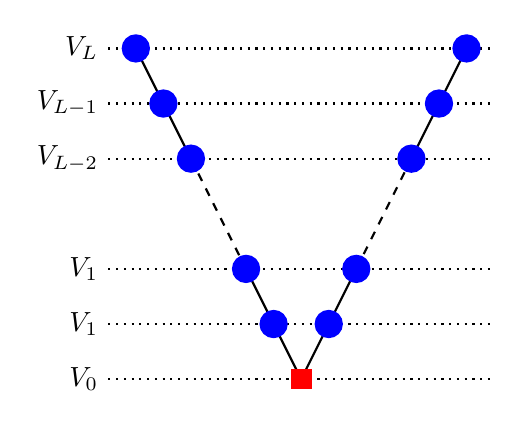
\begin{tikzpicture}[thick,scale=.7]
    % Levels
    \draw[dotted](0,0) node[anchor=east]{$V_0$} -- (7,0);
    \draw[dotted](0,1) node[anchor=east]{$V_1$} -- (7,1);
    \draw[dotted](0,2) node[anchor=east]{$V_1$} -- (7,2);
    \draw[dotted](0,4) node[anchor=east]{$V_{L-2}$} -- (7,4);
    \draw[dotted](0,5) node[anchor=east]{$V_{L-1}$} -- (7,5);
    \draw[dotted](0,6) node[anchor=east]{$V_L$} -- (7,6);
    
    % Transfers
    \draw(0.5,6) -- (1.5,4);
    \draw[dashed](1.5,4) -- (2.5,2);
    \draw(2.5,2) -- (3.5,0) -- (4.5,2);
    \draw[dashed](4.5,2) -- (5.5,4);
    \draw(5.5,4) -- (6.5,6);
    
    % Smoothers and coarse grid correction
    \node at (0.5,6) [circle,draw=blue,fill=blue] {};
    \node at (1.0,5) [circle,draw=blue,fill=blue] {};
    \node at (1.5,4) [circle,draw=blue,fill=blue] {};
    \node at (2.5,2) [circle,draw=blue,fill=blue] {};
    \node at (3.0,1) [circle,draw=blue,fill=blue] {};
    \node at (4.0,1) [circle,draw=blue,fill=blue] {};
    \node at (4.5,2) [circle,draw=blue,fill=blue] {};
    \node at (5.5,4) [circle,draw=blue,fill=blue] {};
    \node at (6.0,5) [circle,draw=blue,fill=blue] {};
    \node at (6.5,6) [circle,draw=blue,fill=blue] {};
    \node at (3.5,0) [rectangle,draw=red,fill=red] {};
  \end{tikzpicture}    
  \end{minipage}
  \begin{minipage}[t]{.49\linewidth}
  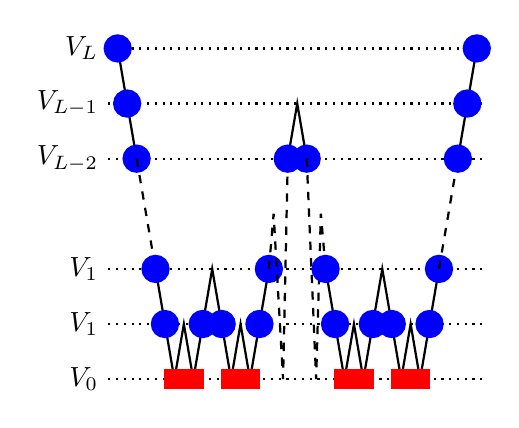
\begin{tikzpicture}[thick,yscale=.7,xscale=.6]
    % Levels
    \draw[dotted](0,0) node[anchor=east]{$V_0$} -- (8.0,0);
    \draw[dotted](0,1) node[anchor=east]{$V_1$} -- (8.0,1);
    \draw[dotted](0,2) node[anchor=east]{$V_1$} -- (8.0,2);
    \draw[dotted](0,4) node[anchor=east]{$V_{L-2}$} -- (8.0,4);
    \draw[dotted](0,5) node[anchor=east]{$V_{L-1}$} -- (8.0,5);
    \draw[dotted](0,6) node[anchor=east]{$V_L$} -- (8.0,6);

    % Transfers and smoothers
    \draw(0.2,6) node[circle,draw=blue,fill=blue] {}
    -- (0.4,5) node[circle,draw=blue,fill=blue] {}
    -- (0.6,4) node[circle,draw=blue,fill=blue] {};
    \draw[dashed](0.6,4) -- (1.0,2);
    \draw (1.0,2) node[circle,draw=blue,fill=blue] {}
    -- (1.2,1) node[circle,draw=blue,fill=blue] {}
    -- (1.4,0) node[rectangle,draw=red,fill=red] {}
    -- (1.6,1)
    -- (1.8,0) node[rectangle,draw=red,fill=red] {}
    -- (2.0,1) node[circle,draw=blue,fill=blue] {}
    -- (2.2,2)
    -- (2.4,1) node[circle,draw=blue,fill=blue] {}
    -- (2.6,0) node[rectangle,draw=red,fill=red] {}
    -- (2.8,1)
    -- (3.0,0) node[rectangle,draw=red,fill=red] {}
    -- (3.2,1) node[circle,draw=blue,fill=blue] {}
    -- (3.4,2) node[circle,draw=blue,fill=blue] {};
    \draw[dashed](3.4,2) -- (3.5,3) -- (3.7,0) -- (3.8,4);
    \draw(3.8,4) node[circle,draw=blue,fill=blue] {}
    -- (4.0,5)
    -- (4.2,4) node[circle,draw=blue,fill=blue] {};
    \draw[dashed] (4.2,4) -- (4.4,0) -- (4.5,3) 
    -- (4.6,2)
    ;
    \draw (4.6,2) node[circle,draw=blue,fill=blue] {}
    -- (4.8,1) node[circle,draw=blue,fill=blue] {}
    -- (5.0,0) node[rectangle,draw=red,fill=red] {}
    -- (5.2,1)
    -- (5.4,0) node[rectangle,draw=red,fill=red] {}
    -- (5.6,1) node[circle,draw=blue,fill=blue] {}
    -- (5.8,2)
    -- (6.0,1) node[circle,draw=blue,fill=blue] {}
    -- (6.2,0) node[rectangle,draw=red,fill=red] {}
    -- (6.4,1)
    -- (6.6,0) node[rectangle,draw=red,fill=red] {}
    -- (6.8,1) node[circle,draw=blue,fill=blue] {}
    -- (7.0,2) node[circle,draw=blue,fill=blue] {};
    \draw[dashed] (7.0,2) -- (7.4,4);
    \draw (7.4,4) node[circle,draw=blue,fill=blue] {}
    -- (7.6,5) node[circle,draw=blue,fill=blue] {}
    -- (7.8,6) node[circle,draw=blue,fill=blue] {};    
  \end{tikzpicture}    
  \end{minipage}
  \caption{Smoothing and grid transfer of the V-cycle (left) and
    W-cycle (right). Black lines indicate grid transfer, blue dots are
  smoothing operations and red squares are coarse grid
  solvers. ``Time'' is left to right.}
  \label{fig:mg:1}
\end{figure}

\begin{remark}
  Figure~\ref{fig:mg:1} shows that the recursive structure of the
  W-cycle is much more complex than that of the V-cycle. The
  complexity analysis below will show that higher values of
  $m_{\text{coarse}}$ do not lead to efficient algorithms.
\end{remark}

\begin{definition}
  If the numbers of pre- and post smoothing steps in the V-cycle are
  dependent on the level $\ell$, we speak of the \define{variable
    V-cycle}. A typical choice is $m_\ell = 2^{L-\ell} m_L$, thus
  doubling the number of smoothing steps whenever stepping down one
  level.
\end{definition}

\begin{note}
  The variable V-cycle with $m_\ell$ as mentioned in the previous
  definition has as many smoothing steps per iteration as the W-cycle.
\end{note}

\begin{remark}
  If we use an additive or multiplicative Schwarz method (omitting the
  coarse grid) as our smoother $R_\ell$, it should be possible in
  principle to use the analytical tools of
  Chapter~\ref{cha:iteration:schwarz-methods}. The difficulty then
  consists in ensuring that the spectral radius of the iteration
  matrix does not grow towards one if we proceed upwards on our scale
  of spaces $V_\ell$. This remark is a todo for the author and an
  encouragement for the reader. Hints may be found
  in~\cite{GriebelOswald95,Xu92}.
\end{remark}

\begin{remark}
  It turns out that the techniques used for the analysis of the
  V-cycle and the W-cycle, respectively are quite
  different. Therefore, we separate them into two sections.
\end{remark}

\begin{theorem}
  Let $n_\ell$ be the dimension of $V_\ell$. Assume that the effort
  needed to for the operations in equations~\eqref{eq:mg:5}b/c/e is
  linear in $n_\ell$ and assume that $ n_{\ell+1}/n_\ell \approx 2^d$,
  where $d$ is the space dimension of the grid. Assume that the effort
  for the coarse grid solver is negligible. Then, the effort for
  one step of the V-cycle is of order $n_L$. The effort for one step
  of the W-cycle is of order $n_L$ for $d \ge 2$, while it is of order
  $n_L \log(n_L)$ in one dimension.
\end{theorem}

\begin{proof}
  Start the recursion on level $L$ with the function $MG_L(0,
  g)$. This function calls $MG_{L-1}(\ldots)$ $m_{\text{coarse}}$
  times. Thus, by recursion, $MG_{\ell}(\ldots)$ is executed
  $m_{\text{coarse}}^{L-\ell}$ times.
  
  By our assumptions, the amount of operations $\breve N_\ell$ in $MG_\ell(\ldots)$
  without the coarse grid correction is linear in $n_\ell$, say
  bounded by $Cn_\ell$. Then, the overall effort $N_L$ on level $L$ is
  \begin{gather}
    \label{eq:mg:6}
    N_L \le C \sum_{\ell=1}^L n_\ell m_{\text{coarse}}^{L-\ell} \le C
    \sum_{\ell=1}^L n_L 2^{d(l-L)}m_{\text{coarse}}^{L-\ell}
    = C n_L \sum_{\ell=1}^L \left(\frac{m_{\text{coarse}}}{2^d}\right)^l.
  \end{gather}
  It remains to notice that the sum converges and is bounded
  independent of $L$ if and only if $m_{\text{coarse}}/2^d < 1$.
\end{proof}

\begin{lemma}
  Let $B_\ell^{-1}$ be the operator associated with the action of the
  multigrid preconditioner on level $\ell$ for
  $\ell=0,\ldots,L$. Then, the error after one step of the multigrid
  method has the form
  \begin{gather}
    \label{eq:mg:7}
    u^{(k+1)} - u = E_L \left(u^{(k)} - u \right),
  \end{gather}
  where for $\ell=0,\ldots,L$ we denote by $E_\ell$ the
  \putindex{error propagation operator}
  \begin{gather}
    \label{eq:mg:8}
    E_\ell = \left(I-R_\ell^{-1} A_\ell\right)^{m_{\text{post}}}
    \left(I-B_{\ell-1}^{-1}A_{\ell-1} P_{\ell-1}\right)^{m_{\text{coarse}}}
     \left(I-R_\ell^{-1} A_\ell\right)^{m_{\text{pre}}}
  \end{gather}
\end{lemma}

\begin{proof}
  For the smoother, we use the standard technique for Richardson's
  method outlined in Lemma~\ref{lemma:richardson:1}.
\end{proof}


\section{The V-cycle}

\section{The W-cycle and two-grid convergence}


%%% Local Variables: 
%%% mode: latex
%%% TeX-master: "main"
%%% End: 


\printbibliography
\printindex
\end{document}


%%% Local Variables: 
%%% mode: latex
%%% TeX-master: "main"
%%% End: 
